\documentclass[12pt,oneside]{report}

% Paquetes necesarios
\usepackage{times}          % Fuente Times New Roman
\usepackage{setspace}       % Control de interlineado
\usepackage[margin=2.5cm]{geometry} % Márgenes de 2.5 cm
\usepackage{fancyhdr}       % Encabezados y pies de página
\usepackage{titlesec}       % Control de títulos
\usepackage{tocloft}        % Control de tabla de contenidos
\usepackage[spanish,es-tabla]{babel}
\usepackage{ragged2e}
\justifying{}
\usepackage{microtype}
\usepackage{graphicx}   % para \includegraphics
\usepackage{float}      % para [H] en figuras y tablas
\usepackage{pdflscape}  % páginas apaisadas (diagrama de la metodología)
\usepackage{afterpage}  % coloca la página apaisada sin dejar la anterior a medias
\usepackage{eso-pic}    % número de página de la hoja apaisada
% Página apaisada: el número se coloca abajo al centro de la vista apaisada (borde
% derecho de la hoja), girado como el contenido, en lugar del pie normal.
\newcommand{\numeroapaisado}{\thispagestyle{empty}%
  \AddToShipoutPictureFG*{\AtPageLowerLeft{\put(\LenToUnit{\paperwidth-1.45cm},\LenToUnit{0.5\paperheight}){%
    \makebox(0,0){\rotatebox{90}{\thepage}}}}}}
\usepackage{booktabs}   % para tablas de mejor calidad (\toprule, \midrule, \bottomrule)
\usepackage{caption}    % para control de leyendas
\captionsetup{justification=justified, singlelinecheck=false} % leyendas justificadas a la izquierda
\usepackage{subcaption} % para subfiguras si se necesitan
\usepackage{amsmath}
\usepackage{xcolor}
\usepackage[spanish]{todonotes}  % comentarios de revisión (retirar en la versión final)
% Comentario de revisión en el cuerpo del texto
\newcommand{\comentario}[1]{\todo[inline, color=red!8, bordercolor=red, linecolor=red]{\small #1}}
% Configuración de interlineado
\onehalfspacing
% Source - https://tex.stackexchange.com/a/73865
% Posted by alamodey
% Retrieved 2026-05-26, License - CC BY-SA 2.5
\usepackage{comment} 

\usepackage{hyperref}
\hypersetup{
    colorlinks,
    citecolor=black,
    filecolor=black,
    linkcolor=black,
    urlcolor=black
}

% Configuración de numeración de páginas
\pagestyle{fancy}
\fancyhf{}
\fancyfoot[C]{\thepage}     % Número de página centrado abajo
\setlength{\parindent}{1.27 cm}
\renewcommand{\headrulewidth}{0 pt}
\renewcommand{\footrulewidth}{0 pt}
% Opcional: formato de capítulos y secciones
\titleformat{\chapter}[display]
  {\normalfont\bfseries\centering}
  {\Huge\chaptername\ \thechapter}{20pt}{\Huge}

% Rutas de figuras: las del documento y las generadas por el código
\graphicspath{{figuras/}{../resultados/figuras/}}

% Documento
\begin{document}

\newpage
\pagestyle{empty}
\mbox{}
\newpage

% Portada
\begin{titlepage}
    \centering
    {\huge \textbf{Interpretación Física del Comportamiento Electromagnético de Nanocompuestos SWCNT/Poliimida Basado en Imágenes KPFM y Aprendizaje Automático} \par}
    \vspace{4.5 cm}
    {\huge Sergio David Colmenares Socha \par}
    \vspace{.2 cm}
    {\large \textbf{Director:} Octavio Alejandro Castañeda Uribe \par}
    
    {\large \textbf{Codirector:} Jose Augusto Galvis Echeverry \par}
    \vspace{3.5 cm}
    
    {\large Trabajo para el Grado en: \par}
    
    {\Large \textbf{\textit{Ingeniería Electrónica}} \par}
    \vspace{1 cm}
    \vfill
    
    {\large Colegio Mayor Nuestra Señora del Rosario \par}

    {\large Escuela de Ciencias e Ingeniería \par}
    
    
    {\large Bogotá, Colombia \par}
    {\large 2026 \par}
\end{titlepage}


\newpage
\pagestyle{empty}
\mbox{}
\newpage




\newpage

\chapter*{Resumen}


\vspace{0.5cm}
\noindent\textbf{Palabras clave:}
\thispagestyle{empty}


\chapter*{Abstract}


\vspace{0.5cm}
\noindent\textbf{Keywords:}
\thispagestyle{empty}

\newpage
\setcounter{page}{1}
\pagestyle{empty}
\mbox{}
\newpage



% Tabla de contenidos
\pagestyle{fancy}
\tableofcontents
\newpage

\listoffigures
\addcontentsline{toc}{chapter}{Lista de Figuras}
\newpage
 
\listoftables
\addcontentsline{toc}{chapter}{Lista de Tablas}
\newpage

% Aquí empieza el contenido principal


% Capítulos
\chapter{Introducción}
En las últimas décadas, la ciencia de materiales ha presentado transformaciones significativas impulsadas especialmente por los avances en nanotecnología. Esta disciplina, capaz ya no solo de analizar, sino también de diseñar y estructurar materiales en escalas invisibles al ojo humano haciendo uso de nuevas y diferentes técnicas, tiene como objetivo configurar propiedades de los mismos de manera controlada. Esto constituye una revolución en un mundo que exige más y más soluciones específicas a problemas complejos en diferentes ámbitos, en los cuales el estudio de nanomateriales tiene un papel importante a desempeñar.

Bajo este contexto, este trabajo se engloba en un tipo específico de nanomaterial, los polímeros nanocompuestos. Estos están construidos a partir de matrices poliméricas sobre las cuales se integra material nanoparticulado. Existen muchos tipos y configuraciones de los mismos, buscando en ellos diferentes características, definidas por las variables usadas en su fabricación y aplicación: el tipo de polímero y nanorelleno utilizado, concentraciones, métodos de unión, entre muchas otras cuestiones que hacen que cada composición varíe sus propiedades respecto a otras y a sus propios componentes.

Con el objetivo de obtener propiedades que sean útiles en muchos campos; desde el ámbito académico, pasando por la industria y el desarrollo militar, hasta soluciones en el campo de la salud y en materia ambiental: constantemente se están planteando, estudiando y manufacturando nuevos tipos de polímeros nanocompuestos.  

Una de las características de mayor interés en este tipo de materiales es la eficiencia de apantallamiento (SE) frente a interferencia electromagnética (EMI). Los dispositivos electrónicos actuales requieren materiales que los protejan del ruido externo y preserven la integridad de las señales que manejan. La proliferación de sistemas que operan en bandas de alta frecuencia ha incrementado los requerimientos de apantallamiento [12], tanto por la mayor facilidad con que los sistemas se acoplan con señales parásitas en ese régimen como por los estándares de compatibilidad electromagnética (EMC). Para aplicaciones prácticas, se considera un umbral de referencia de aproximadamente 20 dB de SE como requisito para aplicaciones comerciales [4]. 

Frente a esto, la tarea de diseñar polímeros nanocompuestos capaces de aislar los sistemas de este tipo de ruido es crucial, pues aporta ventajas estructurales, económicas y de otros tipos, frente a aislamientos convencionales. La interacción de las nanopartículas con las ondas electromagnéticas es lo que permite el apantallamiento, mientras que el polímero se encarga del manejo estructural y contribuye indirectamente en la absorción o el reflejo de la interferencia electromagnética [1], [12].

En este trabajo se realizó un análisis sobre nanocompuestos SWCNT/poliimida, con el objetivo de dar una interpretación física a la relación del apantallamiento electromagnético de diferentes muestras medido a partir de parámetros S, por medio del uso de descriptores morfológicos propuestos y medibles sobre los datos de las mismas. Estos datos son obtenidos a partir de microscopía de Fuerza de Sonda Kelvin de Segundo Armónico (KPFM) [5], capaz de realizar la medición del gradiente de capacitancia $\partial C/\partial z$ en cada posición. Son representaciones de la muestra en formato de imagen y sobre las mismas se realiza la medición de descriptores. La búsqueda de relaciones entre los descriptores y la medición de efectividad de apantallamiento (SE) se realiza usando modelos de Machine Learning (ML), capaces de detectar las características más influyentes en la propiedad de interés a partir de modelos predictivos e interpretables.

Con base en lo expuesto, la pregunta de investigación que dirige este proyecto es: ¿Cuáles son los descriptores morfológicos de la red de SWCNTs, extraídos de imágenes KPFM, que se relacionan cuantitativamente con la eficacia de apantallamiento electromagnético del nanocompuesto? La hipótesis es que la morfología de la red, caracterizada a partir de las imágenes de gradiente de capacitancia, determina en parte significativa el SE del material, y que modelos de ML interpretables pueden identificar y jerarquizar esa relación.

Si bien no es nueva la caracterización de muestras a partir de descriptores apuntando a la relación con SE, realizada en el trabajo de Castañeda Uribe y Avila [4], usando tres descriptores morfológicos (CNTD, CNTA, CNTS) y parámetros S, la conexión sistemática con la morfología de la red no está completamente establecida en este tipo de nanocompuestos. 

Este trabajo extiende esta línea a partir de tres enfoques:(i) un conjunto ampliado de descriptores morfológicos, soportado por un pipeline de procesamiento de imágenes diseñado para extraerlos de forma robusta y generalizada; (ii) un espacio experimental con mayor variabilidad en las condiciones de fabricación; y (iii) la integración de modelos de ML interpretables para identificar y jerarquizar los descriptores que se relacionan con el SE, habilitando su posterior interpretación física. 

El enfoque del trabajo busca evitar caracterizaciones cualitativas, fundamentando el análisis físico a proponer. Se reconocen limitaciones en cuanto a la cantidad de muestras y a la proyección 2D de la red tridimensional, derivada del procesamiento de imágenes. De resultar efectivo, se podría generalizar este proceso para el análisis de muestras de nanocompuestos poliméricos similares.

\section{Objetivos}
\label{sec:objetivos}
El objetivo general de este trabajo es analizar la relación entre descriptores morfológicos obtenidos a partir de imágenes de distribuciones de nanotubos de carbono (CNTs) y la eficacia de apantallamiento electromagnético en nanocompuestos poliméricos de CNT/poliimida, mediante el uso de modelos de inteligencia artificial interpretables y mediciones experimentales de parámetros S. Para ello se plantean los siguientes objetivos específicos:
\begin{itemize}

\item Aplicar técnicas de procesamiento digital de imágenes para reducir el ruido de imágenes obtenidas por KPFM, con el fin de mejorar el contraste entre los nanotubos de carbono y la matriz polimérica.
\item Extraer descriptores morfológicos físicamente interpretables a partir de las imágenes filtradas, que representen cuantitativamente la distribución espacial de los CNTs en la matriz.
\item Entrenar modelos de inteligencia artificial explicables utilizando los descriptores morfológicos como variables de entrada y las eficacias de apantallamiento electromagnético, obtenidas mediante parámetros S, como variable objetivo.
\item Interpretar la influencia de la morfología interna de los nanocompuestos en su eficacia de apantallamiento electromagnético, empleando descriptores morfológicos extraídos de imágenes de caracterización para explicar el comportamiento del material desde una perspectiva fundamentada en la física del electromagnetismo y de los semiconductores.
\end{itemize}

\chapter{Marco Teórico}
Este capítulo busca contextualizar al lector en la interdisciplinariedad del trabajo. Se pretende explicar el trasfondo teórico de las diferentes áreas articuladas en el estudio. Se hace un recorrido sobre los componentes y técnicas de cada etapa del proyecto: Una revisión de los polímeros nanocompuestos, un estudio de la técnica de microscopía de fuerza atómica(AFM) usada para la medición del gradiente de capacitancia sobre las muestras, un análisis del procesamiento digital del conjunto de imágenes, la caracterización de los descriptores propuestos, una descripción del SE y parámetros S como variable objetivo del estudio, y finalmente una revisión de los modelos de ML aplicables en el problema.

\section{Polímeros Nanocompuestos}
Estos tipos de nanocompuestos son materiales fabricados a partir de matrices poliméricas a las que se les agregan diversos tipos de nanorelleno. Este nanorelleno está compuesto por partículas que poseen al menos una dimensión geométrica en el orden de los nanómetros. La mayor ventaja que tienen estos nanocompuestos es que logran combinar las propiedades de la matriz y de las nanopartículas, para que funcionen en conjunto y potencien características que individualmente no se expresan [10]. Esto abre un amplio espacio de posibilidades para sus diferentes configuraciones. Desde enfoques en características eléctricas, o en propiedades mecánicas, químicas, e incluso biomédicas.

Existen gran variedad de nanopartículas que pueden ser usadas en la configuración de estos materiales. Diferentes geometrías, composiciones y propiedades de base. Además de esas diferentes especificaciones iniciales, en el proceso de fabricación también surgen otras características que pueden ser configurables para modificar en mayor o menor medida las propiedades finales del compuesto. Entre ellas están la concentración, dispersión, conectividad, entre muchas otras variables. Precisamente aquí es donde surgen varios de los descriptores propuestos.

Dado que la caracterización se realiza sobre la red de CNTs, es fundamental conocer sus características individuales, que son el fundamento de las características generales de la red. Los nanocompuestos con los que se trabaja en este estudio son SWCNTs, nanotubos de carbono de pared simple formados a partir de grafeno enrollado en forma de cilindro, sobre la matriz de poliimida. El diámetro es de 1 $nm$ típicamente [3], y su longitud en orden de micrómetros. Basado en la interacción del CNT, se puede establecer el comportamiento eléctrico del mismo. Este comportamiento y el del polímero, son los que permiten medir las redes a partir del contraste del gradiente de capacitancia.

\section{Gradiente de Capacitancia: KPFM}
\label{sec:kpfm}

La microscopía de Fuerza Atómica AFM es una técnica de microscopía a nivel nanométrico capaz de realizar mediciones de características topográficas de muestras a partir de la interacción entre su superficie y la punta nanométrica del microscopio. El método consiste en el barrido oscilatorio de la punta sobre la muestra, a medida que recorre las irregularidades de la superficie, el cantiléver presenta deflexiones que provocan que un haz de luz reflejado en la punta se modifique y al captar esas variaciones topográficas, se ajusta la altura para mantener la amplitud de resonancia.

Basado en este método, se han desarrollado variaciones del mismo, capaces de medir otras propiedades de las muestras. La microscopía de Fuerza de Sonda Kelvin de Segundo Armónico añade la medición de características eléctricas. El método específico consiste en 2 pasadas sobre la muestra. La primera obtiene la medición topográfica a partir de la técnica AFM. La segunda pasada, mide la vibración inducida por la interacción eléctrica entre la punta y la muestra generada por una señal de voltaje AC aplicada en la punta, ahora a altura fija sobre la topografía. El segundo armónico de esta vibración es proporcional con el gradiente de capacitancia $\partial C/\partial z$, que contiene la información subsuperficial de la muestra, como describe [5]. Esta medición, como bien se dice, no es infalible, dada la pérdida de definición de los CNTs más profundos, explicada por la difusión de las líneas de campo eléctrico en el trayecto punta-CNT.

\subsubsection{Implicación}
En números, la detección en profundidad se ve limitada a $\approx 430 nm$ [5]. Conociendo la complejidad geométrica tridimensional de los datos; y por simplicidad del análisis para la extracción de la red de CNTs, esta se considerará coplanar y se proyectarán las estructuras sobre un plano 2D. Se asume que todas las regiones detectadas influyen equitativamente sobre el SE, a pesar de las deformaciones y pérdida de resolución generadas por la detección en profundidad. Esta delimitación se establece reconociendo que pueden existir métodos de reconstrucción tridimensional de la red no usados, pues su implementación queda fuera del alcance de este trabajo.

\section{Procesamiento Digital de Imágenes}
Después de obtenidos los datos, estos pueden ser visualmente analizados en formato de imagen.  Al hacer una revisión inicial del conjunto de imágenes, se puede concluir que son un grupo heterogéneo que presenta diferenciaciones dadas tanto en sus condiciones de fabricación, como por la adquisición de datos a partir de la técnica de microscopía ya mencionada. Esto último es visualmente claro y denota uno de los problemas principales del estudio. 

La extracción de la red de nanotubos representa una gran dificultad pues se pretende crear un pipeline estándar de procesamiento de imágenes capaz de cubrir todos los casos presentes en un conjunto de este tipo. Esta es una tarea compleja dado que no solo hay que tener en cuenta la variabilidad de los datos en cuanto a distribución de CNTs, especialmente CNTs subsuperficiales, cuyo contraste obtenido por el gradiente de capacitancia los hace matemáticamente indistinguibles del fondo. Sino que se le suma la presencia de múltiples tipos de ruido en los datos obtenidos.

El pipeline debe ser capaz de atacar el ruido presente en cada muestra, evitando modificar la morfología de la red. El desarrollo del mismo debe ser cuidadoso puesto que es un proceso sin ajustes individuales o manuales para un conjunto heterogéneo, buscando la esca labilidad a conjuntos de datos más grandes. Se esperan resultados funcionales de extracción de redes de gradiente $\partial C/\partial z$ a pesar de los parámetros generales aplicados a todas las imágenes. 

El tratamiento que se debe hacer a cada imagen según el ruido presente en la misma debe ser cuidadoso porque el procesamiento es general para todos los datos y no se tiene un ajuste manual por muestra.

Si se cumple con estos dos apartados, tanto la obtención de la red como la minimización del ruido de forma aceptable, se tiene una base sólida para el cálculo de descriptores; en otro caso se podrían ignorar regiones de nanotubos profundos, o que surjan falsos positivos al crear artefactos basados en el ruido, ensuciando los datos que alimentaran al modelo.

\subsection{Caracterización del Ruido}
Por medio de análisis visual se pudo identificar tres tipos principales de ruido en los datos de microscopía. Estos resultados surgen de un análisis empírico, pero sirven como contextualización de la teoría que respalda el pipeline de limpieza y binarización realizado.

\subsubsection{Crosstalk Topográfico}

Dada la referencia topográfica que sigue la técnica AFM, es posible visualizar en la imagen del gradiente de capacitancia, artefactos superficiales o de ruido inducidos por la medición superficial. Esto es un problema muy presente en el dataset, puesto que hay imágenes eléctricas con relieves y rayones, o peor aún, imágenes eléctricas donde cambios topográficos muy abruptos causan que, en la medición, la punta pierda contacto o presente deflexiones no surgidas del gradiente de capacitancia. Cuando ocurre esto, aparecen regiones donde la información del gradiente es nula o poco confiable. Estos casos son problemáticos puesto que el error del crosstalk está muy presente en el dataset. La gran mayoría de las manchas y rayones encontrados, entre otras manifestaciones de ruido presuntamente aleatorio, son en realidad función sistemática de la presencia de la topografía en el canal eléctrico, inherente a la técnica de microscopía. En resumen, tanto superficie como ruido captado en la señal topográfica se ven introducidos en la señal eléctrica con el agravante de que el gradiente es en mayor magnitud sensible a la distancia [8].

\begin{figure}[H]
    \centering
    \begin{minipage}{0.35\textwidth}
        \centering
        \includegraphics[width=\textwidth]{1c-6_sh.png}
        \includegraphics[width=\textwidth]{0a-5_sh.png}
    \end{minipage}
    \begin{minipage}{0.35\textwidth}
        \centering
        \includegraphics[width=\textwidth]{1c-6_topo.png}
        \includegraphics[width=\textwidth]{0a-5_topo.png}
    \end{minipage}
    \caption{Crosstalk: Imágenes del Canal Eléctrico (Izquierda). Imágenes del Canal Topográfico (Derecha).}
    \label{fig:comparacion}
\end{figure}

\subsubsection{Ruido Impulsivo}
Este tipo de ruido aleatorio se presenta con frecuencia tanto en forma de píxeles con valores extremos (Outliers), como en filas totales o parciales también afectadas por el mismo fenómeno de valores extremos. este tipo de ruido se debe a interferencias mecánicas o eléctricas en la medición [8].

\begin{figure}[H]
    \centering
    \includegraphics[width=0.35\textwidth]{0a-4_sh.png}
    \caption{Visualización de Filas, Píxeles y Regiones con Valores Extremos (Zoom).}
    \label{fig:etiqueta}
\end{figure}
\subsubsection{Artefactos de Barrido}
Los artefactos de Barrido, y otros tipos de ruido sistemático horizontal se presentan debido a la deriva de temperatura, cambios en las propiedades de la punta, en la electrónica de adquisición, o dada la diferencia temporal de escaneo entre filas. Se presenta como variaciones de fondos que no corresponden a la realidad física [8].

\begin{figure}[H]
    \centering
    \includegraphics[width=0.35\textwidth]{0b-5_sh.png}
    \caption{Artefactos de Escaneo.}
    \label{fig:etiqueta}
    
\end{figure}


\section{Caracterización de Descriptores}
Los descriptores son herramientas de medición de características sobre la información visual de las muestras, con las cuales se adquieren propiedades relevantes de la red de nanotubos, que serán usados para la predicción de SE a partir de ML. 

A continuación, se definen los grupos de descriptores.
\subsection{Distribución Espacial}
La separación entre regiones conductoras dentro de la matriz condiciona la formación de caminos continuos y la fracción de área disponible para reflejar y absorber ondas electromagnéticas. Espaciados uniformes favorecen redes regulares; espaciados desiguales o aglomeraciones generan zonas con concentraciones distintas de portadores [4]. Los descriptores de este grupo cuantifican estas características mediante CNTD, CNTA y CNTS.

\subsection{Intensidad de Gradiente}
La intensidad del gradiente de capacitancia $\partial C/\partial z$ responde a la densidad local de CNTs y a su proximidad a la superficie [4]. Dado que las ondas electromagnéticas inciden desde la superficie, las regiones con valores altos tienen mayor peso relativo en la reflexión y en la primera capa de absorción [5]. Los descriptores de este grupo cuantifican la magnitud y variabilidad espacial del gradiente sobre la red segmentada.

\subsection{Forma y Morfología}
La geometría de los segmentos detectados condiciona la respuesta conductora de la red. El área cuantifica el tamaño de cada región conductora local. La elongación caracteriza la forma del agrupamiento, indicando si los CNTs internos tienden a estar alineados o distribuidos de forma isotrópica. La curvatura cuantifica el grado de tortuosidad del agrupamiento, asociado a la interconexión interna de sus CNTs. Estas propiedades modulan la efectividad de los agrupamientos como elementos conductores de la red [1].

\subsection{Orientación}
La interacción entre una onda electromagnética polarizada y un CNT depende del ángulo entre el eje del nanotubo y el campo eléctrico, por lo que la direccionalidad preferencial de la red modula la respuesta del material [4]. En este trabajo la orientación se mide sobre el esqueleto de los agrupamientos detectados, asumiendo que normalmente la dirección del esqueleto refleja la orientación interna de los CNTs cuando éstos tienden a estar localmente alineados. Los descriptores de este grupo capturan la orientación dominante de la red y el grado de coherencia direccional.

\subsection{Conectividad y Topología}
La capacidad de un nanocompuesto de apantallar ondas electromagnéticas depende de la formación de caminos conductores continuos. La teoría de percolación establece un umbral crítico de concentración por encima del cual la red se vuelve macroscópicamente conductora [2]. Los descriptores de este grupo cuantifican la fracción ocupada por el clúster mayor, la longitud total de la red y su grado de fragmentación.

\subsection{Perfil de Gradiente}
En varias imágenes se observa una tendencia global del gradiente a lo largo del eje vertical de barrido, cuyo origen puede ser un artefacto residual del procesamiento o un efecto físico real asociado a la organización en profundidad. Dado que su origen no puede determinarse con la información disponible, los descriptores de este grupo se incluyen como elementos exploratorios.

\section{SE y Parámetros S}
La eficiencia de apantallamiento electromagnético (SE) es la variable objetivo sobre la cual se busca establecer una relación cuantitativa con los descriptores morfológicos extraídos de las imágenes KPFM. Descrita como la medición de la capacidad de un material de aislar o atenuar señales electromagnéticas normalmente consideradas ruido. 
Este trabajo parte de los valores de SE ya obtenidos a partir de parámetros S y centra su aporte en la etapa posterior a la adquisición; los detalles de la medición se encuentran descritos en [4].

\subsection{Parámetros S}
Los parámetros S describen el comportamiento de un material en términos de su respuesta a señales electromagnéticas, esta descripción se basa en ondas incidentes, reflejadas y transmitidas. Específicamente $S_{11}$ cuantifica la fracción de onda incidente reflejada en la interfaz, y $S_{21}$ la fracción transmitida. A partir de sus magnitudes se derivan tres cantidades que describen el apantallamiento [4]:

    $$SE_R = 10 \log_{10}\left(\frac{1}{1 - |S_{11}|^2}\right)$$

$$SE_A = 10 \log_{10}\left(\frac{1 - |S_{11}|^2}{|S_{21}|^2}\right)$$

$$SE_T = SE_R + SE_A$$

$SE_R$ corresponde a la atenuación por reflexión en la superficie; $SE_A$ corresponde a la atenuación por absorción dentro del volumen del material,
asociada a pérdidas dieléctricas y conductivas; $SE_T$ es la
atenuación total.

Cada mecanismo responde de forma distinta a la organización de
los CNTs: la reflexión depende de la conductividad superficial
(redes percolantes cerca de la superficie), mientras que la
absorción depende de la densidad de caminos conductores en el
volumen [1], [12]. En CNT/poliimida, el mecanismo dominante es la absorción [3], [4]. Esta diferenciación motiva a analizar los tres mecanismos por separado contra los descriptores morfológicos.


\section{Modelos de ML}
Con los datos obtenidos a partir de los descriptores y los datos SE, el siguiente paso es su análisis profundo por medio de Machine Learning. 

El Aprendizaje de Máquina es una de las ramas de la Inteligencia Artificial enfocada en el desarrollo de algoritmos capaces de encontrar patrones en los datos. Los modelos suelen clasificarse según la interacción entre las variables de los datos en modelos supervisados, si existe una variable objetivo con resultados predefinidos, o no supervisado, si los modelos analizan conjuntos de datos sin etiquetas.

Los modelos supervisados se usan esencialmente para la resolución de dos tipos específicos de problemas, regresión y clasificación. En este trabajo se aplican diferentes modelos supervisados buscando: 

Un análisis predictivo de la relación entre los descriptores y mediciones de SE usando modelos de regresión y con gran interpretabilidad, con el objetivo de dar interpretación física a las relaciones de los descriptores más influyentes.

Un análisis exploratorio de clasificación intentando detectar patrones en los descriptores que permitan agrupar las muestras a partir de sus características de fabricación. 

\subsection{Interpretabilidad}
Dado que el objetivo del proyecto es no solo observar cuáles son los descriptores con más peso en los modelos, sino aparte de eso buscar darles una interpretación física válida, es fundamental que los modelos usados presenten siempre gran interpretabilidad.
Esta característica no es más sino la capacidad de entender cómo y por qué el modelo toma las decisiones que lo llevan a sus diferentes predicciones, atribuyendo de esta forma significado a los pesos asignados a las variables de entrada que justifican los descriptores más influyentes.


\subsection{Modelos para Regresión}

\subsubsection{Ridge}
Modelo de regresión lineal con regularización L2. Penaliza la magnitud cuadrada de los coeficientes, lo que reduce el sobre ajuste cuando hay variables correlacionadas y produce coeficientes estables. Los coeficientes resultantes son directamente interpretables como peso lineal de cada descriptor en la predicción [7].


\subsubsection{Lasso} 
Modelo de regresión lineal con regularización L1. La penalización tiene la propiedad de llevar coeficientes de variables poco informativas exactamente a cero, lo que efectivamente realiza selección de variables. Esta característica es particularmente útil en este trabajo, donde el número de descriptores (20) puede contener variables redundantes o irrelevantes [7].


\subsubsection{Random Forest}
Modelo basado en el promedio de múltiples árboles de decisión, cada uno entrenado con subconjuntos aleatorios de datos y variables. Captura relaciones no lineales e interacciones entre variables que los modelos lineales no pueden representar. Su interpretabilidad se obtiene a través de la importancia de variables y, complementariamente, mediante importancia por permutación [7].

\subsection{Modelos para Clasificación}

\subsubsection{Random Forest Classifier} 
Variante de clasificación del modelo descrito anteriormente, con la misma estrategia de árboles ensamblados aplicada a etiquetas categóricas. Permite identificar qué descriptores son más relevantes para distinguir entre condiciones de fabricación [7].

\subsubsection{Análisis discriminante lineal (LDA)} 
Método de clasificación que proyecta el espacio de variables sobre las direcciones que maximizan la separación entre categorías y minimizan la varianza interna de cada una. Asume distribuciones gaussianas con igual covarianza entre clases. Su utilidad principal en este trabajo es de visualización y diagnóstico: permite verificar si las condiciones de fabricación son linealmente separables en el espacio de descriptores [7].


\chapter{Metodología}

Este capítulo describe los procedimientos aplicados sobre el conjunto de datos de microscopía de fuerza electrostática de segundo armónico (EFM-2$\omega$) empleado en este trabajo. La descripción se organiza en torno a los objetivos específicos del proyecto (Sección~\ref{sec:objetivos}), registrando la metodología aplicada en aquellos en que sea necesaria, con el fin de asegurar la claridad y reproducibilidad del trabajo. Estos objetivos son: el procesamiento digital de los datos de microscopía para reducir el ruido y aumentar el contraste de la red de nanotubos respecto a la matriz polimérica, la extracción de descriptores morfológicos físicamente interpretables a partir de las matrices procesadas y los procedimientos de ML enfocados en la relación SE-descriptores.

La Figura~\ref{fig:met_panorama} resume la metodología en seis etapas. Cada operación recibe una o varias matrices y entrega una nueva; sus nombres se indican en la figura y se definen en la Tabla~\ref{tab:nomenclatura}. El propósito de cada etapa es el siguiente:

\begin{enumerate}
    \item \textbf{Adquisición.} De cada medición se extraen el canal eléctrico $E_0$ y el canal topográfico $H_0$.
    \item \textbf{Preprocesamiento.} Corrige, uno a uno, los defectos del canal eléctrico que complicarían separar la red del fondo. Primero, ambos canales se llevan a una escala común mediante una normalización robusta, que no se ve afectada por los valores extremos del ruido y permite compararlos ($\tilde E$, $\tilde H$). Con ellos se corrige el crosstalk topográfico: las huellas de la topografía en el canal eléctrico, como bordes de rayones y partículas, que reducen el contraste entre los CNTs y el fondo ($E_{\mathrm{CT}}$). Un filtro de sal y pimienta reemplaza después los píxeles aislados con valores extremos, que la segmentación podría clasificar como red ($E_{\mathrm{SP}}$). Como el microscopio adquiere la matriz línea por línea y el nivel de base de la señal se desplaza durante el barrido, cada línea tiene un nivel de fondo propio, que en la imagen aparece como bandas horizontales; la corrección de fondo por línea resta a cada línea su nivel ($E_{\mathrm{BG}}$). Esta corrección resta un único valor por línea, por lo que no corrige los desplazamientos que afectan solo a un tramo de ella; esos tramos se eliminan con un filtro que compara cada píxel con los de las líneas superiores e inferiores ($E_{\mathrm{FL}}$). Por último, cada medición se escala al intervalo $[0,1]$, de modo que los umbrales de la segmentación tengan el mismo significado en todas las mediciones ($E_{\mathrm{seg}}$).
    \item \textbf{Extracción de máscara.} Clasifica cada píxel como red o como fondo. Como los CNTs se encuentran a distintas profundidades, la intensidad de su señal varía; por ello se combinan tres binarizaciones de distinta escala espacial que se compensan entre sí: la local capta el detalle de la red, y la regional y la global descartan el fondo que la local confunde con red. Si la combinación resulta demasiado restrictiva, se emplea la binarización local como respaldo. El resultado es la máscara final $M_{\mathrm{F}}$.
    \item \textbf{Matrices para la extracción de descriptores.} El cierre morfológico repara las discontinuidades que la segmentación introduce en la red ($M_{\mathrm{C}}$), y la esqueletización la reduce a su eje central, sobre el que se miden longitudes y trayectorias ($S$).
    \item \textbf{Extracción de descriptores.} Sobre $M_{\mathrm{F}}$, $M_{\mathrm{C}}$ y $S$ se calculan 13 descriptores por medición, agrupados según la característica de la red que cuantifican. Los de distribución espacial (CNTD, CNTA y CNTS) miden, a partir de líneas de barrido simuladas sobre $M_{\mathrm{C}}$, si los CNTs se reparten con espaciados regulares o se concentran en aglomeraciones. Los de forma (área media y su desviación, elongación y tortuosidad) describen el tamaño de las regiones de la red, cuán alargadas son y cuánto se desvían sus estructuras de una trayectoria recta. Los de orientación (ángulo dominante y coherencia) indican si la red sigue una dirección preferente y con qué grado de alineación. Los de conectividad (cobertura, índice de percolación, longitud de red y número de fragmentos) evalúan qué fracción de la superficie ocupa la red, en qué medida forma una estructura continua y cuán extensa es. Los valores de las 81 mediciones forman la matriz de descriptores $X$, de $81\times13$.
    \item \textbf{Análisis de resultados.} La matriz $X$ se relaciona con la eficacia de apantallamiento (SE) mediante un análisis exploratorio y modelos interpretables.
\end{enumerate}

Las etapas 1 a 4 se describen en la Sección~\ref{sec:met_procesamiento}, la etapa 5 en la Sección~\ref{sec:met_descriptores} y la etapa 6 en la Sección~\ref{sec:met_analisis}.

\afterpage{%
\begin{landscape}\numeroapaisado
\begin{figure}[p]
\centering
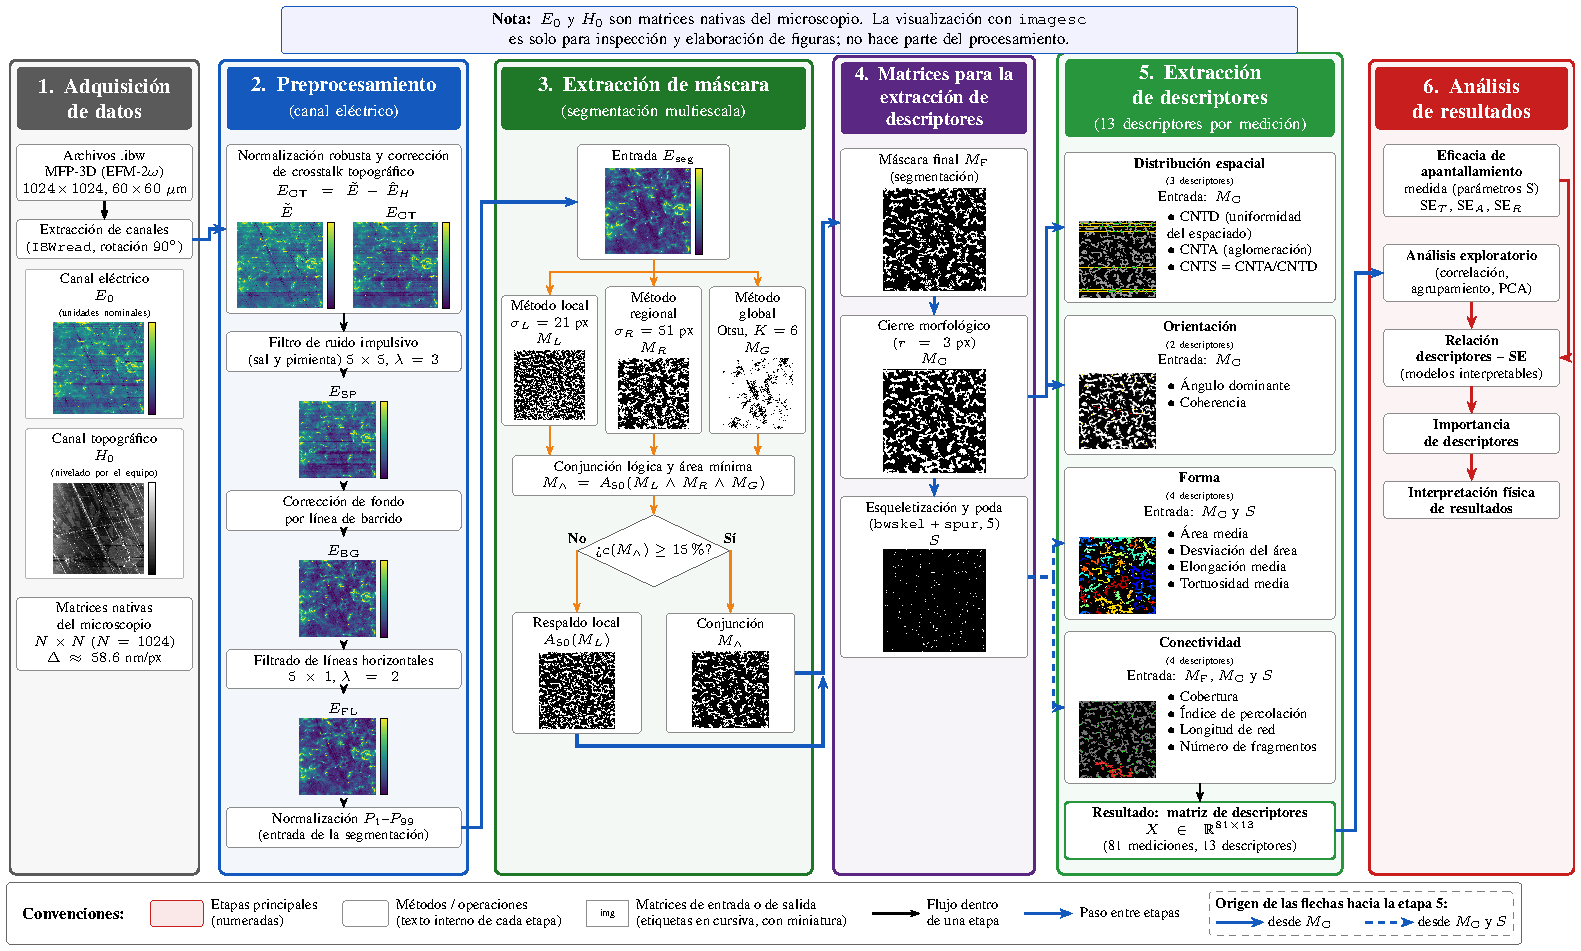
\includegraphics[width=\linewidth]{diagrama_metodologia.pdf}
\caption{Panorama general de la metodología. Las miniaturas corresponden a la medición 0a-5; la escala de color de cada matriz se fija en sus percentiles 1 y 99, y cada miniatura cubre el área de barrido completa, de $60\times60~\mu$m.}
\label{fig:met_panorama}
\end{figure}
\end{landscape}
}

Los nombres de las matrices siguen una convención: $E$ designa el canal eléctrico; $H$, la altura topográfica; $M$, una máscara binaria; $S$, el esqueleto; y $X$, la matriz de descriptores. El subíndice 0 indica los datos originales; la tilde, la normalización robusta; el acento circunflejo, un valor estimado mediante un ajuste; y los subíndices en letra recta, la operación que produce la matriz (por ejemplo, CT: corrección de crosstalk; BG: corrección de fondo, del inglés \emph{background}).

\begin{table}[H]
\centering
\caption{Nomenclatura de las matrices de la metodología. La columna ``Se obtiene de'' indica las matrices de entrada de la operación que produce cada una.}
\label{tab:nomenclatura}
\small
\begin{tabular}{@{}l p{7.4cm} l l@{}}
\toprule
\textbf{Símbolo} & \textbf{Descripción} & \textbf{Se obtiene de} & \textbf{Sección} \\
\midrule
$E_0$ & Canal eléctrico original (unidades nominales) & Archivo .ibw & \ref{sec:met_procesamiento} \\
$H_0$ & Canal topográfico original & Archivo .ibw & \ref{sec:met_procesamiento} \\
$\tilde E$, $\tilde H$ & Canales eléctrico y topográfico normalizados por mediana y MAD & $E_0$, $H_0$ & \ref{sec:met_crosstalk} \\
$\hat E_H$ & Componente del canal eléctrico estimada a partir de la topografía & $\tilde E$, $\tilde H$ & \ref{sec:met_crosstalk} \\
$E_{\mathrm{CT}}$ & Canal eléctrico corregido de crosstalk & $\tilde E$, $\hat E_H$ & \ref{sec:met_crosstalk} \\
$E_{\mathrm{SP}}$ & Canal eléctrico filtrado de ruido impulsivo & $E_{\mathrm{CT}}$ & \ref{sec:met_syp} \\
$E_{\mathrm{BG}}$ & Canal eléctrico corregido de fondo por línea de barrido & $E_{\mathrm{SP}}$ & \ref{sec:met_fondo} \\
$E_{\mathrm{FL}}$ & Canal eléctrico filtrado de líneas horizontales & $E_{\mathrm{BG}}$ & \ref{sec:met_lineas} \\
$E_{\mathrm{seg}}$ & Canal eléctrico normalizado entre $P_1$ y $P_{99}$, en $[0,1]$ & $E_{\mathrm{FL}}$ & \ref{sec:met_norm} \\
$M_L$, $M_R$, $M_G$ & Máscaras de las binarizaciones local, regional y global & $E_{\mathrm{seg}}$ & \ref{sec:met_binarizacion} \\
$M_\wedge$ & Conjunción de $M_L$, $M_R$ y $M_G$, con área mínima por componente & $M_L$, $M_R$, $M_G$ & \ref{sec:met_binarizacion} \\
$M_{\mathrm{F}}$ & Máscara final: $M_\wedge$ o, si se activa el respaldo, la máscara local con área mínima & $M_\wedge$, $M_L$ & \ref{sec:met_binarizacion} \\
$M_{\mathrm{C}}$ & Máscara morfológica, tras el cierre morfológico & $M_{\mathrm{F}}$ & \ref{sec:met_representaciones} \\
$S$ & Esqueleto podado de la red & $M_{\mathrm{C}}$ & \ref{sec:met_representaciones} \\
$X$ & Matriz de descriptores, de $81\times13$ & $M_{\mathrm{F}}$, $M_{\mathrm{C}}$, $S$ & \ref{sec:met_descriptores} \\
\bottomrule
\end{tabular}
\end{table}

\section{Procesamiento Digital de Imágenes}
\label{sec:met_procesamiento}
Las mediciones de microscopía se obtienen en formato .ibw (Igor Binary Wave), el formato de salida del microscopio MFP-3D (Asylum Research) con el que fueron adquiridas. Estos archivos contienen múltiples canales de información adquiridos durante el escaneo EFM-2$\omega$; cada canal es una matriz de $N\times N$ valores reales, con $N = 1024$, que cubre un área de barrido de $60\times60$~$\mu$m. Cada elemento de la matriz se denomina píxel, y la resolución espacial es de $\Delta = 60~\mu\text{m}/1024 \approx 58.6$~nm por píxel. En este trabajo se emplean dos canales: el canal eléctrico $E_0$, que corresponde a la amplitud del segundo armónico de la vibración del cantiléver y es proporcional al gradiente de capacitancia $\partial C/\partial z$ [5], y el canal topográfico $H_0$, que recoge las mediciones de altura de la superficie de la muestra.

El conjunto de datos está formado por 81 mediciones: nueve condiciones de fabricación, resultado de combinar tres voltajes (5, 10 y 15~V) y tres frecuencias (10~Hz, 1~kHz y 100~kHz) [4], con tres réplicas por condición y tres posiciones de medición por réplica. Cada medición se identifica con un código de la forma \texttt{Vf-n}: \texttt{V} indica el voltaje (0, 1 y 2 para 5, 10 y 15~V, respectivamente), \texttt{f} la frecuencia (a, b y c para 10~Hz, 1~kHz y 100~kHz, respectivamente) y $n \in \{1, \dots, 9\}$ la medición, de modo que las mediciones 1--3, 4--6 y 7--9 corresponden a la primera, segunda y tercera réplica, respectivamente. El conjunto de las nueve mediciones de una condición de fabricación se denomina \emph{set}; por ejemplo, el set 2b corresponde a 15~V y 1~kHz.

Ambos canales se extraen del archivo .ibw en MATLAB con la función \texttt{IBWread}, que emplea las funciones auxiliares \texttt{readIBWheaders} y \texttt{readIBWbinheader} para leer los encabezados del archivo [ref. pendiente]. Cada matriz extraída se rota $90^\circ$ (\texttt{rot90}), de modo que su orientación coincida con la que presenta el software del microscopio, en la que cada fila de la matriz corresponde a una línea de barrido. Cada matriz contiene valores reales y no una imagen digital en sentido estricto, cuyos valores estarían cuantizados en niveles de gris; sin embargo, al estar organizada como una función bidimensional discreta de la posición, admite las operaciones de procesamiento digital de imágenes [6], cuya terminología se adopta en este capítulo. Las filas se indexan con $i$ (eje $y$), las columnas con $j$ (eje $x$, a lo largo de la línea de barrido), y los parámetros espaciales se expresan en píxeles (1~px $= \Delta \approx 58.6$~nm). El valor de una matriz genérica $Y$ en el píxel de la fila $i$ y la columna $j$, con $i, j \in \{1, \dots, N\}$, se denota $Y(i,j)$. El canal topográfico se guarda nivelado por defecto por el software de adquisición del microscopio, mediante un nivelado de primer orden por línea de barrido: a los valores de altura de cada fila $i$ se ajusta por mínimos cuadrados una recta en función de la columna, $\hat a_i + \hat b_i\, j$, que se resta de la fila. De este modo, si $h(i,j)$ denota la altura registrada antes de la nivelación, el canal guardado es $H_0(i,j) = h(i,j) - (\hat a_i + \hat b_i\, j)$. La nivelación elimina el desnivel ($\hat a_i$) y la inclinación ($\hat b_i$) de cada línea respecto a las demás, pero no las variaciones de orden superior a lo largo de la línea. El canal eléctrico, en cambio, se guarda sin nivelar. La sensibilidad de la detección del segundo armónico no se calibró durante la adquisición, por lo que el canal eléctrico se expresa en unidades nominales: es proporcional al valor real con un factor desconocido, constante dentro de cada medición pero no necesariamente entre sesiones de medición.

La visualización de los canales topográfico y eléctrico se hace con el propósito de inspeccionar cada etapa del procesamiento y construir las figuras de este documento; es un proceso paralelo al procesamiento y no interviene en ningún cálculo. Para esto se usa la función \texttt{imagesc} de MATLAB con ejes de igual escala (\texttt{axis image}), de modo que cada píxel se dibuja como un cuadrado de $\Delta$ de lado. Cada píxel se representa con un color del mapa de color \emph{viridis} (256 colores), asignado según su valor. La asignación es lineal entre dos límites: para las matrices de valores continuos, sus percentiles 1 y 99, de modo que los valores fuera de ese rango toman el color del extremo correspondiente; para las máscaras binarias, los valores 0 y 1. Salvo que se indique lo contrario en la figura, los límites se calculan por separado para cada matriz, por lo que los colores de dos figuras distintas no son comparables entre sí.

A lo largo del procesamiento se emplean dos estadísticos de orden, la mediana y el percentil, sobre un conjunto de valores $x$, por ejemplo todos los píxeles de una matriz o todos los de una fila. La mediana, $\mathrm{med}(x)$, es el valor central del conjunto ordenado, o el promedio de los dos valores centrales si el número de valores es par. El percentil $q$, $P_q(x)$, es el valor por debajo del cual se encuentra el $q$~\% de los valores; se calcula con la función \texttt{prctile} de MATLAB, que interpola linealmente entre los valores ordenados.

Las secciones siguientes describen las operaciones de la Figura~\ref{fig:met_panorama} en el mismo orden en que se aplican: las del preprocesamiento (Secciones~\ref{sec:met_crosstalk} a \ref{sec:met_norm}), la extracción de máscara (Sección~\ref{sec:met_binarizacion}) y la construcción de las matrices para la extracción de descriptores (Sección~\ref{sec:met_representaciones}).

\subsection{Corrección de Crosstalk Topográfico}
\label{sec:met_crosstalk}

Como primera etapa se elimina el crosstalk topográfico [8], es decir, la aparición en el canal eléctrico de rasgos de la topografía de la superficie, como bordes de rayones y partículas. La corrección busca identificar la parte del canal eléctrico que reproduce la topografía y retirarla.

Ambos canales se normalizan primero de forma robusta, restando su mediana y dividiendo por su desviación absoluta mediana (MAD):

\begin{equation}
\begin{gathered}
\tilde E(i,j) = \frac{E_0(i,j) - \mathrm{med}(E_0)}{\mathrm{MAD}(E_0)}, \qquad
\tilde H(i,j) = \frac{H_0(i,j) - \mathrm{med}(H_0)}{\mathrm{MAD}(H_0)}, \\[4pt]
\mathrm{MAD}(x) = \mathrm{med}\left(\left|x - \mathrm{med}(x)\right|\right)
\end{gathered}
\label{eq:norm_robusta}
\end{equation}

donde $\tilde E$ y $\tilde H$ son los canales eléctrico y topográfico normalizados (la tilde indica normalización), adimensionales y comparables entre sí, y la mediana y la MAD de cada canal se calculan sobre todos los píxeles de la matriz. Se emplean la mediana y la MAD en lugar de la media y la desviación estándar porque no se ven afectadas por valores extremos derivados del ruido.

Con los canales normalizados se ajusta un modelo de regresión lineal múltiple que estima la contribución de la topografía a la señal eléctrica. El modelo supone que esta contribución es una combinación lineal de la altura local y de sus variaciones en las direcciones horizontal y vertical:

\begin{equation}
\tilde E(i,j) = \beta_0 + \beta_1 \tilde H(i,j) + \beta_2 \frac{\partial \tilde H}{\partial x}(i,j) + \beta_3 \frac{\partial \tilde H}{\partial y}(i,j) + \varepsilon(i,j)
\label{eq:crosstalk}
\end{equation}

donde $\beta_0, \dots, \beta_3$ son los coeficientes del modelo; $\varepsilon(i,j)$ es el residuo, es decir, la parte de $\tilde E(i,j)$ que las variables topográficas no explican; y $\partial \tilde H/\partial x$ y $\partial \tilde H/\partial y$ son las variaciones direccionales de la topografía, calculadas por diferencias centrales (función \texttt{gradient} de MATLAB):

\begin{equation}
\frac{\partial \tilde H}{\partial x}(i,j) = \frac{\tilde H(i,j+1) - \tilde H(i,j-1)}{2}, \qquad
\frac{\partial \tilde H}{\partial y}(i,j) = \frac{\tilde H(i+1,j) - \tilde H(i-1,j)}{2}
\label{eq:diferencias}
\end{equation}

expresadas por píxel; en la primera y la última columna (o fila) se usa la diferencia de un solo lado, por ejemplo $\tilde H(i,2) - \tilde H(i,1)$.

El modelo se ajusta una sola vez por medición, sobre la matriz completa: cada uno de los $N^2 = 1\,048\,576$ píxeles aporta una ecuación de la forma (\ref{eq:crosstalk}), de modo que se dispone de $N^2$ observaciones para estimar cuatro coeficientes, comunes a toda la medición. Los coeficientes se estiman por mínimos cuadrados, es decir, como los valores $\hat\beta_0, \dots, \hat\beta_3$ que minimizan la suma de los residuos al cuadrado sobre todos los píxeles:

\begin{equation}
(\hat\beta_0, \dots, \hat\beta_3) = \arg\min_{\beta_0, \dots, \beta_3} \sum_{i=1}^{N} \sum_{j=1}^{N} \varepsilon(i,j)^2
\label{eq:minimos_cuadrados}
\end{equation}

donde el acento circunflejo indica un valor estimado a partir de los datos. Este problema se resuelve con el operador \texttt{\textbackslash} de MATLAB, mediante factorización QR. Con los coeficientes estimados se construye la componente del canal eléctrico explicada por la topografía:

\begin{equation}
\hat E_H(i,j) = \hat\beta_0 + \hat\beta_1 \tilde H(i,j) + \hat\beta_2 \frac{\partial \tilde H}{\partial x}(i,j) + \hat\beta_3 \frac{\partial \tilde H}{\partial y}(i,j)
\label{eq:crosstalk_ajuste}
\end{equation}

Aunque los coeficientes son los mismos en toda la medición, la topografía y sus derivadas cambian de un píxel a otro, por lo que $\hat E_H$ es una matriz de $N\times N$ con un valor distinto en cada píxel; el subíndice $H$ indica que corresponde a la parte atribuida a la topografía. Esta matriz se resta píxel a píxel del canal eléctrico normalizado:

\begin{equation}
E_{\mathrm{CT}}(i,j) = \tilde E(i,j) - \hat E_H(i,j)
\label{eq:crosstalk_resta}
\end{equation}

La matriz $E_{\mathrm{CT}}$ contiene los residuos del ajuste y es la entrada de las etapas siguientes. La corrección elimina la parte del canal eléctrico asociada linealmente con la topografía y sus derivadas; sin embargo, no distingue entre los artefactos instrumentales y las variaciones eléctricas que se correlacionan físicamente con la morfología de la superficie.

Por construcción de los mínimos cuadrados, $E_{\mathrm{CT}}$ tiene media nula y correlación nula con $\tilde H$ y con sus derivadas, por lo que la correlación posterior a la corrección no mide su efectividad. Por esta razón, el efecto de la corrección se examina visualmente, comparando para una misma medición el canal topográfico, el canal eléctrico normalizado $\tilde E$ y el canal corregido $E_{\mathrm{CT}}$, con atención a las huellas topográficas, como bordes de rayones y partículas superficiales. La Figura~\ref{fig:met_crosstalk} muestra esta comparación para la medición 0a-5.

\begin{figure}[H]
\centering
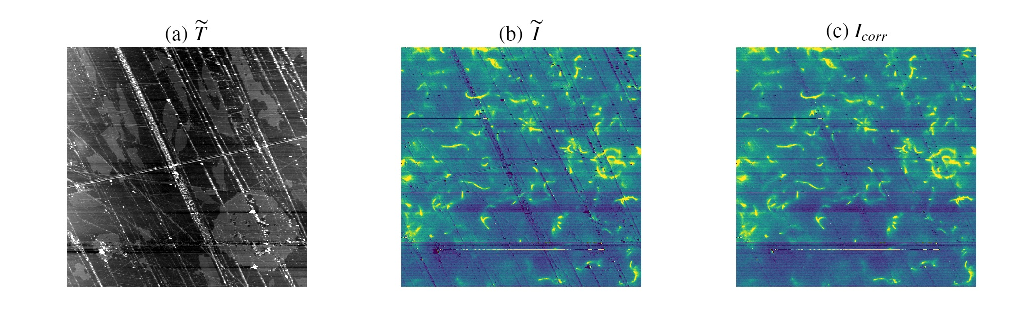
\includegraphics[width=\textwidth]{metodologia/met_crosstalk.pdf}
\caption{Corrección de crosstalk topográfico en la medición 0a-5. (a) Canal topográfico normalizado $\tilde H$, en escala de grises. (b) Canal eléctrico normalizado $\tilde E$. (c) Canal corregido $E_{\mathrm{CT}}$. Los paneles (b) y (c) comparten los límites de color, fijados en los percentiles 1 y 99 de $\tilde E$.}
\label{fig:met_crosstalk}
\end{figure}


\subsection{Filtrado de Ruido Impulsivo}
\label{sec:met_syp}

Para eliminar el ruido impulsivo se emplea un filtro de mediana bidimensional [6] aplicado de forma selectiva. El filtro se describe para una matriz de entrada genérica $Y$ y una ventana (kernel) de $a\times b$ píxeles ($a$ filas por $b$ columnas, ambos impares); en esta etapa, $a = b = 5$. El procedimiento tiene tres pasos.

Primero, la ventana se centra en cada píxel $(i,j)$ y abarca el conjunto de píxeles

\begin{equation}
W_{a\times b}(i,j) = \left\{ (u,v) : |u - i| \le \tfrac{a-1}{2},\ |v - j| \le \tfrac{b-1}{2} \right\}
\label{eq:ventana}
\end{equation}

esto es, el píxel central y los píxeles situados a una distancia de hasta $(a-1)/2$ filas y $(b-1)/2$ columnas de él. El filtro de mediana asigna a cada píxel la mediana de los $a\cdot b$ valores de su ventana:

\begin{equation}
Y_{med}(i,j) = \mathrm{med}\left\{ Y(u,v) : (u,v) \in W_{a\times b}(i,j) \right\}
\label{eq:mediana}
\end{equation}

En los bordes de la matriz, las posiciones de la ventana que quedan fuera se completan con ceros (comportamiento por defecto de la función \texttt{medfilt2} de MATLAB). La mediana es insensible a los propios outliers: un valor aislado extremo queda en un extremo del conjunto ordenado y no modifica el valor central, propiedad que la hace adecuada para la eliminación de ruido impulsivo.

Segundo, sobre el residuo $R(i,j) = Y(i,j) - Y_{med}(i,j)$ obtenido entre la matriz previa $Y$ y la posterior al filtro $Y_{med}$ se estima la desviación típica del ruido, $\hat\sigma_{SyP}$, mediante un estimador robusto basado en la mediana absoluta, calculado una sola vez con todos los píxeles de la matriz:

\begin{equation}
\hat\sigma_{SyP} = \frac{\mathrm{med}(|R|)}{0.6745}
\label{eq:mad}
\end{equation}

El factor $0.6745$ es el percentil 75 de la distribución normal estándar, $\Phi^{-1}(0.75)$, donde $\Phi$ es su función de distribución acumulada: si el residuo de los píxeles sin outliers sigue una distribución normal de media cero y desviación estándar $\sigma_0$, la mitad de los valores de $|R|$ es menor que $0.6745\,\sigma_0$, es decir, la mediana de $|R|$ vale $0.6745\,\sigma_0$. En consecuencia, el cociente (\ref{eq:mad}) estima $\sigma_0$ sin verse afectado por los outliers, mientras estos sean menos de la mitad de los píxeles.

Tercero, los píxeles cuyo residuo supera $\lambda$ veces dicha estimación, con $\lambda$ un umbral fijado para cada instancia del filtro, se reemplazan por el valor del filtro de mediana; el resto conserva su valor original. El resultado del filtro es

\begin{equation}
Y_{out}(i,j) =
\begin{cases}
Y_{med}(i,j), & |R(i,j)| > \lambda\,\hat\sigma_{SyP} \\
Y(i,j), & \text{en otro caso}
\end{cases}
\label{eq:impulsivo}
\end{equation}

De este modo, a diferencia de un filtro de mediana convencional, solo se modifican los píxeles anómalos y el resto de la matriz conserva su resolución.

En esta etapa el filtro se aplica con $Y = E_{\mathrm{CT}}$, inmediatamente después de la corrección de crosstalk, con ventana $5\times5$ y umbral $\lambda=3$, para eliminar outliers tipo sal y pimienta (SyP); el resultado $Y_{out}$ se denota $E_{\mathrm{SP}}$. El mismo filtro se reutiliza más adelante, con otra ventana y otro umbral, para eliminar líneas impulsivas horizontales (Sección~\ref{sec:met_lineas}). La Figura~\ref{fig:met_syp} ilustra esta etapa sobre la medición 0c-2.

\begin{figure}[H]
\centering
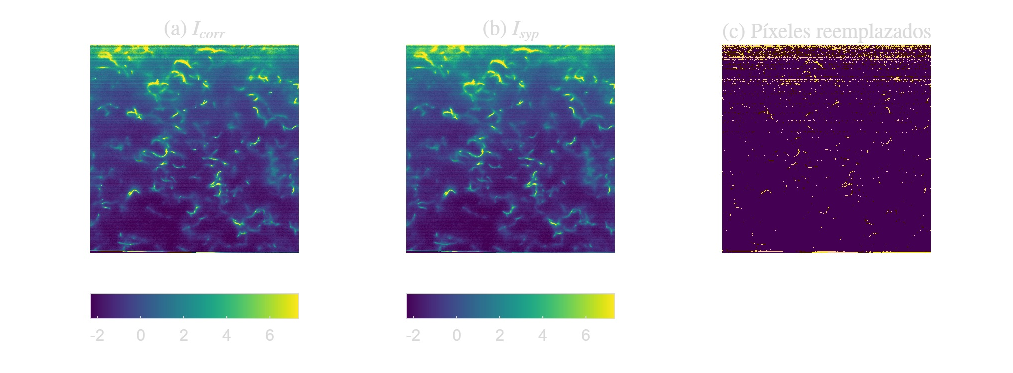
\includegraphics[width=\textwidth]{metodologia/met_syp.pdf}
\caption{Filtrado de ruido impulsivo en la medición 0c-2. (a) Matriz de entrada $E_{\mathrm{CT}}$. (b) Resultado $E_{\mathrm{SP}}$. (c) Píxeles reemplazados por el valor del filtro de mediana. Los paneles (a) y (b) comparten los límites de color.}
\label{fig:met_syp}
\end{figure}


\subsection{Corrección de Fondo por Línea de Barrido}
\label{sec:met_fondo}

Tras la corrección de crosstalk y la limpieza de outliers, se ajusta el nivel de cada fila para eliminar los desplazamientos de nivel entre líneas de barrido derivados del proceso de escaneo [8]. Para cada fila se asume que los píxeles de menor intensidad representan el fondo polimérico, ya que los CNTs aparecen como valores altos del gradiente de capacitancia. Se analiza el vector de intensidad de la fila $i$ de $E_{\mathrm{SP}}$, $\mathbf{f}_i = \left(E_{\mathrm{SP}}(i,1), \dots, E_{\mathrm{SP}}(i,N)\right)$, cuyo elemento $j$ se denota $f_i(j)$, y se calcula un índice de variabilidad relativa:

\begin{equation}
\rho_i = \frac{\mathrm{MAD}(\mathbf{f}_i)}{P_{95}(\mathbf{f}_i) - P_{5}(\mathbf{f}_i)}
\label{eq:rho}
\end{equation}

donde $\mathrm{MAD}(\mathbf{f}_i)$ es la desviación absoluta mediana de la fila, definida en (\ref{eq:norm_robusta}), y $P_{95}(\mathbf{f}_i)$ y $P_{5}(\mathbf{f}_i)$ son sus percentiles 95 y 5. Este índice define de forma adaptativa el percentil $q_i$ (en porcentaje) de píxeles utilizados para estimar el fondo, acotado entre el 25~\% y el 45~\%. El nivel de fondo $b_i$ de la fila es la mediana de los píxeles cuyo valor no supera el percentil $P_{q_i}(\mathbf{f}_i)$, y se resta a la fila completa:

\begin{equation}
\begin{gathered}
q_i = \min\left(45,\ \max\left(25,\ 40 - 20\,\rho_i\right)\right), \\[4pt]
b_i = \mathrm{med}\left\{ f_i(j) : f_i(j) \le P_{q_i}(\mathbf{f}_i) \right\}, \\[4pt]
E_{\mathrm{BG}}(i,j) = f_i(j) - b_i
\end{gathered}
\label{eq:fondo}
\end{equation}

Como $\rho_i \ge 0$, el percentil nunca supera el 40~\%, y la cota inferior solo se alcanzaría con $\rho_i \ge 0.75$. Para las distribuciones de intensidad esperables en una fila (fondo con ruido y una fracción de CNTs de hasta la mitad de la fila), $q_i$ queda aproximadamente entre el 32~\% y el 39~\%: el fondo de cada fila se estima con aproximadamente el tercio de menor intensidad de sus píxeles. El percentil disminuye en las filas con una fracción alta de CNTs (distribución bimodal), en las que un percentil mayor incluiría píxeles de la red en la estimación del fondo. La Figura~\ref{fig:met_fondo} ilustra esta etapa sobre la medición 2a-1.

\begin{figure}[H]
\centering
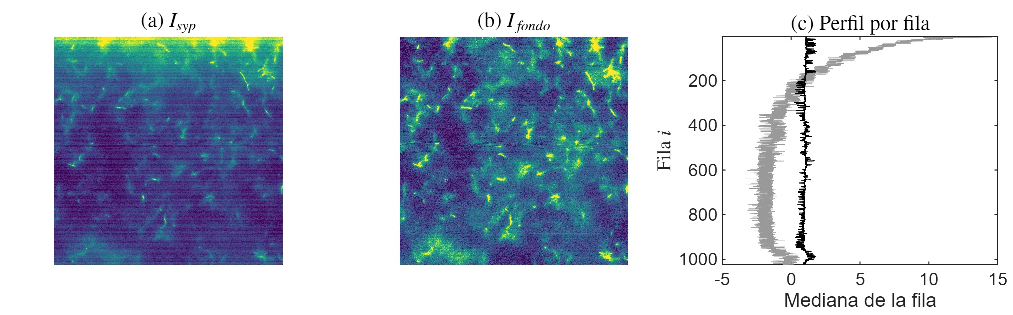
\includegraphics[width=\textwidth]{metodologia/met_fondo.pdf}
\caption{Corrección de fondo por línea de barrido en la medición 2a-1. (a) Matriz de entrada $E_{\mathrm{SP}}$. (b) Resultado $E_{\mathrm{BG}}$. (c) Mediana de cada fila antes (gris) y después (negro) de la corrección, en función de la fila $i$.}
\label{fig:met_fondo}
\end{figure}


\subsection{Filtrado de Líneas Horizontales}
\label{sec:met_lineas}

Tras la corrección de fondo pueden permanecer tramos de línea de barrido cuyo nivel difiere del de las líneas vecinas, que se manifiestan como líneas impulsivas horizontales. Para eliminarlos se aplica nuevamente el filtro de la Sección~\ref{sec:met_syp}, con $Y = E_{\mathrm{BG}}$, una ventana vertical de $5\times1$ ($a = 5$ filas por $b = 1$ columna) y umbral $\lambda=2$; la estimación $\hat\sigma_{SyP}$ de (\ref{eq:mad}) se recalcula para esta instancia. Con esta ventana, cada píxel se compara únicamente con los dos píxeles superiores y los dos inferiores de su misma columna: un tramo de línea desplazado respecto a sus vecinas produce un residuo grande y se reemplaza, mientras que una ventana horizontal no detectaría este defecto, dado que los vecinos del píxel pertenecerían a la misma línea defectuosa. El resultado $Y_{out}$ se denota $E_{\mathrm{FL}}$. La Figura~\ref{fig:met_lineas} ilustra esta etapa sobre la medición 0c-2.

\begin{figure}[H]
\centering
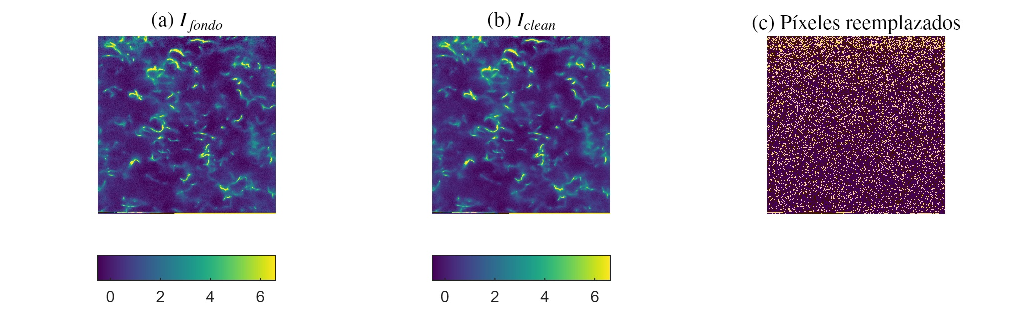
\includegraphics[width=\textwidth]{metodologia/met_lineas.pdf}
\caption{Filtrado de líneas horizontales en la medición 0c-2. (a) Matriz de entrada $E_{\mathrm{BG}}$. (b) Resultado $E_{\mathrm{FL}}$. (c) Píxeles reemplazados por el valor del filtro de mediana con ventana vertical de $5\times1$. Los paneles (a) y (b) comparten los límites de color.}
\label{fig:met_lineas}
\end{figure}


\subsection{Normalización}
\label{sec:met_norm}

Finalmente, se aplica una normalización robusta entre los percentiles 1 y 99 de $E_{\mathrm{FL}}$, $P_1 = P_1(E_{\mathrm{FL}})$ y $P_{99} = P_{99}(E_{\mathrm{FL}})$, calculados sobre todos los píxeles de la matriz, para escalar los datos al intervalo $[0,1]$ y estandarizar el contraste de cara a la binarización:

\begin{equation}
E_{\mathrm{seg}}(i,j) = \max\left(0,\; \min\left(1,\; \frac{E_{\mathrm{FL}}(i,j) - P_{1}}{P_{99} - P_{1}}\right)\right)
\label{eq:norm}
\end{equation}

El 1~\% de valores extremos de cada lado se satura en 0 y en 1, de modo que unos pocos píxeles no dominan la escala de los umbrales de binarización. La matriz resultante se muestra en la Figura~\ref{fig:met_binarizacion}(a).

\subsection{Segmentación Multiescala y Binarización}
\label{sec:met_binarizacion}

Esta etapa separa los píxeles pertenecientes a la red de nanotubos del fondo polimérico. Como los CNTs se encuentran a distintas profundidades dentro del polímero, modificando la señal captada por el microscopio, se requiere un método capaz de detectar tanto regiones superficiales como profundas, manteniendo la morfología y la continuidad espacial de la red, especialmente cuando se presentan cambios de profundidad.

La segmentación se construye como una combinación de tres binarizaciones complementarias sobre $E_{\mathrm{seg}}$: local, global y regional, cuyas máscaras se integran por conjunción. Cada máscara es una matriz de $N\times N$ con valor 1 en los píxeles clasificados como red y 0 en los de fondo.

\subsubsection{Binarización Local}

La instancia local se basa en una umbralización adaptativa con núcleo gaussiano [6], implementada con las funciones \texttt{adaptthresh} e \texttt{imbinarize} de MATLAB. Para cada píxel se estima el fondo local $\mu_{\sigma}(i,j)$ como un promedio ponderado de las intensidades de su vecindad, calculado como la convolución de $E_{\mathrm{seg}}$ con un núcleo gaussiano bidimensional $G_\sigma$ de desviación estándar $\sigma$, lo que asigna mayor peso a los vecinos cercanos al píxel central:

\begin{equation}
\mu_{\sigma}(i,j) = \sum_{|u-i| \le h} \sum_{|v-j| \le h} G_{\sigma}(u-i,\, v-j)\, E_{\mathrm{seg}}(u,v), \qquad
G_{\sigma}(\delta_u, \delta_v) = \frac{1}{Z}\exp\left(-\frac{\delta_u^2 + \delta_v^2}{2\sigma^2}\right)
\label{eq:gauss}
\end{equation}

donde $(\delta_u, \delta_v)$ es el desplazamiento, en píxeles, entre el vecino $(u,v)$ y el píxel central; $h = \lceil 2\sigma \rceil$ es la semianchura del núcleo, que se trunca a $(2h+1)\times(2h+1)$ píxeles; y $Z$ es la suma de los valores de la exponencial dentro de ese soporte, de modo que los pesos suman 1. Los vecinos ubicados fuera de la matriz adoptan el valor del píxel de borde más cercano. En la binarización local, $\sigma = \sigma_L = 21$~px ($\approx 1.2$~$\mu$m), con un núcleo de $85\times85$~px. En \texttt{adaptthresh}, esta desviación estándar corresponde al parámetro \texttt{NeighborhoodSize} con estadístico gaussiano.

Un píxel se clasifica como nanotubo en la máscara local $M_L$ si su intensidad supera la estimación local de fondo escalada por un factor $\gamma$, que depende del parámetro de sensibilidad $s \in [0,1]$ de \texttt{adaptthresh}:

\begin{equation}
M_L(i,j) = \begin{cases} 1, & E_{\mathrm{seg}}(i,j) > \min\left(1,\ \gamma\, \mu_{\sigma_L}(i,j)\right) \\ 0, & \text{en otro caso} \end{cases}, \qquad \gamma = 1.6 - s
\label{eq:bin_local}
\end{equation}

La relación $\gamma = 1.6 - s$ es la que aplica \texttt{adaptthresh} para objetos más brillantes que el fondo (opción \texttt{'ForegroundPolarity','bright'}), y el umbral se acota a 1, el máximo de $E_{\mathrm{seg}}$.

Con $s = 0.55$, $\gamma = 1.05$: un píxel se clasifica como red si su intensidad supera en un 5~\% la media ponderada de su vecindad. Una sensibilidad mayor reduce $\gamma$ y aumenta el número de píxeles clasificados como red. El solapamiento entre las vecindades de píxeles vecinos asegura la continuidad en la captura de variaciones sutiles del gradiente. Esta binarización aporta alta definición pero introduce falsos positivos derivados de pequeñas variaciones eléctricas en el fondo, ya que su criterio es relativo: en zonas de fondo de baja intensidad, una diferencia relativa del 5~\% corresponde a una magnitud absoluta reducida, que el ruido supera con facilidad.

\subsubsection{Binarización Global}

Como complemento, se realiza una binarización global basada en rangos de intensidad mediante una variación del método de Otsu [9] extendida a múltiples clases (\texttt{multithresh}). Dado que la formulación original de dos clases no captura los distintos grupos de intensidades de CNTs presentes en la matriz, se aplica un análisis multinivel que calcula $K = 6$ umbrales $t_1 < \dots < t_6$. Con $t_0 = 0$ y $t_7 = 1$, los umbrales dividen los píxeles de la matriz en siete clases según su valor de $E_{\mathrm{seg}}$, $C_k = \{(i,j) : t_k \le E_{\mathrm{seg}}(i,j) < t_{k+1}\}$ para $k = 0, \dots, 6$ (la última clase incluye también los píxeles con $E_{\mathrm{seg}} = 1$), y se eligen de modo que maximicen la varianza entre clases:

\begin{equation}
(t_1, \dots, t_6) = \arg\max_{t_1 < \dots < t_6} \sum_{k=0}^{K} \omega_k\,(\mu_k - \mu_{tot})^2
\label{eq:otsu}
\end{equation}

donde $\omega_k$ es la fracción de píxeles de la matriz que pertenecen a la clase $C_k$, $\mu_k$ es la intensidad media de esos píxeles y $\mu_{tot}$ es la intensidad media de toda la matriz. La función \texttt{multithresh} resuelve esta maximización sobre el histograma de $E_{\mathrm{seg}}$ con 256 niveles, por lo que los umbrales toman valores múltiplos de $1/255$. La primera clase, que agrupa los valores más bajos de $E_{\mathrm{seg}}$ y corresponde a las zonas más oscuras del fondo polimérico, se descarta de la máscara resultante $M_G$:

\begin{equation}
M_G(i,j) = \begin{cases} 1, & E_{\mathrm{seg}}(i,j) \ge t_1 \\ 0, & \text{en otro caso} \end{cases}
\label{eq:bin_global}
\end{equation}

A diferencia de las binarizaciones adaptativas, este umbral es absoluto y único para toda la matriz, por lo que excluye las zonas de fondo de baja intensidad que la binarización local, por su criterio relativo, clasificaría como red.

\subsubsection{Binarización Regional}

La binarización regional $M_R$ se construye con el mismo principio que la local, según (\ref{eq:gauss}) y (\ref{eq:bin_local}) con la misma sensibilidad, pero empleando un núcleo significativamente mayor: $\sigma = \sigma_R = 51$~px ($\approx 3$~$\mu$m), truncado a $205\times205$~px, de modo que $M_R(i,j) = 1$ si $E_{\mathrm{seg}}(i,j) > \min(1, \gamma\, \mu_{\sigma_R}(i,j))$. Su función es integrar la interacción entre las escalas global y local, y descartar regiones de ruido que las otras instancias no logran filtrar, especialmente en matrices con mayor ruido de origen.

\subsubsection{Integración de Máscaras}

Cada binarización ofrece resultados consistentes pese a la heterogeneidad del dataset, pero presenta limitaciones complementarias: la local aporta definición a costa de ruido granular, la global secciona bien las capas de intensidad pero con baja definición, y la regional opera como filtro espacial intermedio. Las tres máscaras se integran mediante una conjunción lógica:

\begin{equation}
M_\wedge = A_{50}\left(M_G \,\wedge\, M_R \,\wedge\, M_L\right)
\label{eq:bin_conjuncion}
\end{equation}

donde $\wedge$ es la conjunción lógica píxel a píxel (para dos máscaras $M_1$ y $M_2$, $(M_1 \wedge M_2)(i,j) = 1$ solo si $M_1(i,j) = 1$ y $M_2(i,j) = 1$). Solo los píxeles clasificados como red en las tres binarizaciones forman parte de $M_\wedge$. Adicionalmente, se impone una condición de tamaño mínimo por componente conexa. Una componente conexa es un conjunto máximo de píxeles de valor 1 en el que cualquier par puede unirse por una cadena de píxeles de valor 1 vecinos entre sí, considerando vecinos a los 8 píxeles que comparten un lado o una esquina. El operador $A_{50}$ (\texttt{bwareaopen}) elimina (asigna el valor 0 a) las componentes conexas de menos de 50 píxeles ($\approx 0.17$~$\mu$m$^2$) y se aplica a la máscara resultante de la conjunción, para descartar los fragmentos aislados que se forman donde las tres binarizaciones coinciden solo en unos pocos píxeles. En la implementación, el operador se aplica también a $M_G$ antes de la conjunción; este paso no modifica el resultado, ya que toda componente conexa de la conjunción está contenida en una componente conexa de $M_G$, de modo que las componentes de $M_G$ con menos de 50 píxeles solo pueden originar componentes que el operador final elimina.

\subsubsection{Selección de la Máscara Final y Respaldo Local}

La conjunción puede resultar excesivamente restrictiva en algunas mediciones. Para identificar estos casos se emplea la cobertura de una máscara $M$, es decir, la fracción de píxeles clasificados como red:

\begin{equation}
c(M) = \frac{1}{N^2}\sum_{i=1}^{N}\sum_{j=1}^{N} M(i,j)
\label{eq:cobertura}
\end{equation}

La máscara final $M_{\mathrm{F}}$ se selecciona entre la conjunción y la binarización local según la cobertura de la conjunción:

\begin{equation}
M_{\mathrm{F}} =
\begin{cases}
M_\wedge, & c(M_\wedge) \ge 0.15 \\
A_{50}(M_L), & \text{en otro caso}
\end{cases}
\label{eq:bin_final}
\end{equation}

Cuando la cobertura de la conjunción cae por debajo del 15~\%, se activa el respaldo local: la máscara final es la binarización local, con la misma condición de tamaño mínimo empleada en la conjunción. Este mecanismo no introduce un método alternativo con parámetros propios sino que reutiliza el componente local del pipeline. El umbral de $0.15$ se fijó a partir de la inspección de las coberturas obtenidas por la conjunción, como un límite inferior por debajo del cual la máscara deja de representar la red visible en $E_{\mathrm{seg}}$; de este modo, el respaldo actúa únicamente en las mediciones en las que la conjunción resulta excesivamente restrictiva. En el resto de este documento, todas las operaciones posteriores a la segmentación se aplican sobre $M_{\mathrm{F}}$, sea cual sea la máscara seleccionada.

La Figura~\ref{fig:met_binarizacion} ilustra las binarizaciones y su integración sobre la medición 0c-2.

\begin{figure}[H]
\centering
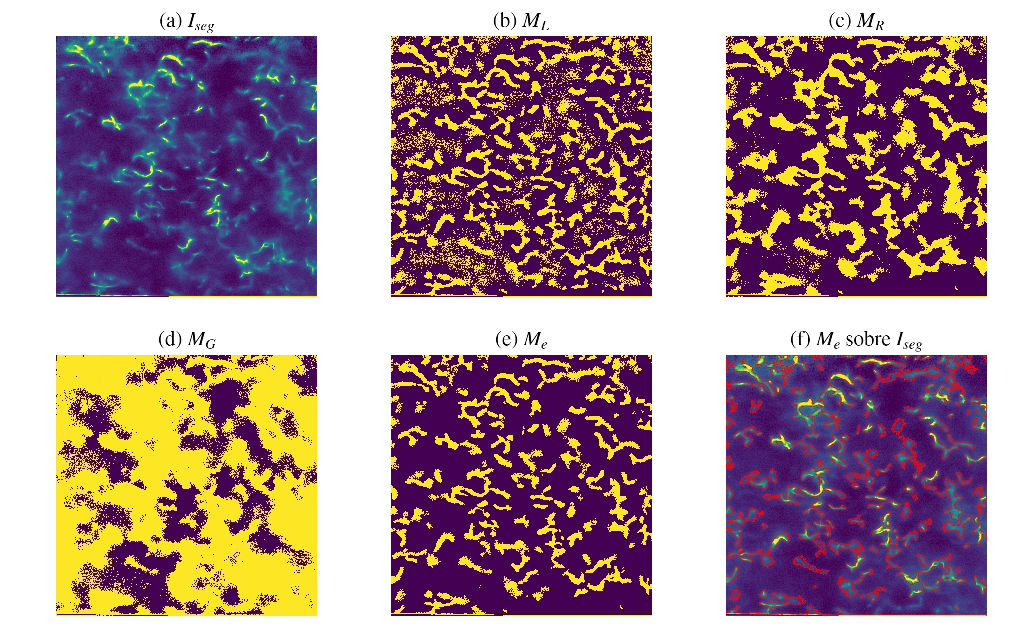
\includegraphics[width=\textwidth]{metodologia/met_binarizacion.pdf}
\caption{Segmentación de la medición 0c-2. (a) Matriz normalizada $E_{\mathrm{seg}}$. (b) Binarización local $M_L$. (c) Binarización regional $M_R$. (d) Binarización global $M_G$. (e) Máscara final $M_{\mathrm{F}}$. (f) Contorno de $M_{\mathrm{F}}$ (rojo) superpuesto a $E_{\mathrm{seg}}$.}
\label{fig:met_binarizacion}
\end{figure}


\subsection{Matrices para la Extracción de Descriptores}
\label{sec:met_representaciones}

A partir de la salida de la segmentación se construyen tres matrices binarias que sirven como insumo común a los distintos grupos de descriptores:

\begin{itemize}
    \item \textbf{Máscara final:} Contiene únicamente los píxeles clasificados como parte de red por la segmentación. Corresponde a $M_{\mathrm{F}}$, definida en (\ref{eq:bin_final}).
    \item \textbf{Máscara morfológica:} Aplica un cierre morfológico sobre la máscara final para unir estructuras y reparar discontinuidades [6]: $M_{\mathrm{C}} = (M_{\mathrm{F}} \oplus B_r) \ominus B_r$, donde $B_r$ es un elemento estructural en forma de disco de radio $r = 3$~px (\texttt{strel('disk',3)}, que MATLAB aproxima mediante una combinación de segmentos lineales), centrado en el origen. Para una máscara genérica $M$, la dilatación $M \oplus B_r$ asigna el valor 1 a todo píxel cuyo disco centrado intersecta al menos un píxel de valor 1 de $M$, lo que engrosa las estructuras y une las que están separadas por huecos estrechos; la erosión $M \ominus B_r$ conserva el valor 1 únicamente en los píxeles cuyo disco centrado está contenido por completo en la región de valor 1, lo que devuelve los bordes exteriores a su posición sin volver a abrir los huecos rellenados. Este radio repara granularidades y recupera continuidades a través de huecos de hasta aproximadamente $2r = 6$~px ($\approx 350$~nm), suficiente para evitar la sobresegmentación de regiones profundas sin destruir la morfología de la red.
    \item \textbf{Esqueleto:} Se obtiene mediante la función \texttt{bwskel} sobre la máscara morfológica. Esta función adelgaza cada componente conexa eliminando de forma iterativa píxeles de sus bordes, sin desconectarla ni abrir o cerrar huecos, hasta reducirla a líneas de 1 px de grosor que siguen su eje central y conservan su topología. Posteriormente se aplican cinco iteraciones de poda de píxeles mediante \texttt{bwmorph(\texttt{'spur'}, 5)}: en cada iteración se eliminan los puntos extremos del esqueleto, es decir, los píxeles con un solo vecino de valor 1 entre sus 8 vecinos. De este modo se recortan progresivamente las ramas y se eliminan las ramas espurias cortas, de hasta aproximadamente 5 px, que aparecen al esqueletizar bordes irregulares, evitando inflar artificialmente los descriptores basados en él. Las ramas largas pierden también hasta 5 px en su extremo libre. El esqueleto resultante se denota $S$.
\end{itemize}

La Figura~\ref{fig:met_representaciones} muestra las matrices para la extracción de descriptores de la medición 0c-2.

\begin{figure}[H]
\centering
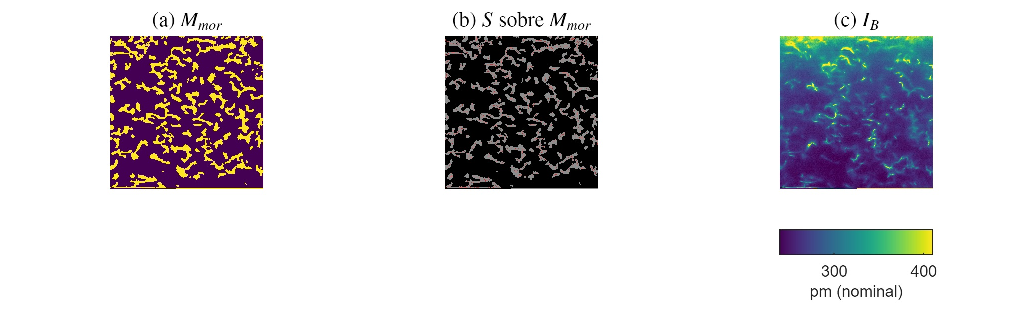
\includegraphics[width=0.67\textwidth]{metodologia/met_representaciones.pdf}
\caption{Matrices para la extracción de descriptores de la medición 0c-2. (a) Máscara morfológica $M_{\mathrm{C}}$. (b) Esqueleto $S$ (rojo) superpuesto a $M_{\mathrm{C}}$ (gris).}
\label{fig:met_representaciones}
\end{figure}


\section{Extracción de Descriptores Morfológicos}
\label{sec:met_descriptores}

Una vez construidas las matrices para la extracción de descriptores (Sección~\ref{sec:met_representaciones}), sobre ellas se calculan 13 descriptores morfológicos por medición, agrupados según la característica de la red que cuantifican: distribución espacial, forma, orientación y conectividad. Cada descriptor resume una medición en un único valor escalar. Todos los descriptores se calculan con la función \texttt{calcular\_descriptores}, desarrollada en MATLAB para este trabajo. La Tabla~\ref{tab:descriptores} resume los 13 descriptores, su símbolo, la matriz sobre la que se calculan y su unidad; los 13 valores de las 81 mediciones forman la matriz de descriptores $X$ (Sección~\ref{sec:met_analisis}).

\begin{table}[H]
\centering
\caption{Descriptores morfológicos calculados por medición.}
\label{tab:descriptores}
\small
\begin{tabular}{@{}l l l l l@{}}
\toprule
\textbf{Grupo} & \textbf{Descriptor} & \textbf{Símbolo} & \textbf{Matriz} & \textbf{Unidad} \\
\midrule
Distribución espacial & Uniformidad del espaciado & CNTD & $M_{\mathrm{C}}$ & adimensional \\
 & Aglomeración & CNTA & $M_{\mathrm{C}}$ & adimensional \\
 & Cociente aglomeración/uniformidad & CNTS & $M_{\mathrm{C}}$ & adimensional \\
\midrule
Forma & Área media de las componentes & $\bar A$ & $M_{\mathrm{C}}$ & $\mu$m$^2$ \\
 & Desviación estándar del área & $s_A$ & $M_{\mathrm{C}}$ & $\mu$m$^2$ \\
 & Elongación media & $\bar e$ & $M_{\mathrm{C}}$ & adimensional \\
 & Tortuosidad media & $\bar\tau$ & $S$ & adimensional \\
\midrule
Orientación & Orientación dominante & $\theta_d$ & $M_{\mathrm{C}}$ & grados \\
 & Coherencia & $\kappa$ & $M_{\mathrm{C}}$ & adimensional \\
\midrule
Conectividad & Cobertura total & $c(M_{\mathrm{F}})$ & $M_{\mathrm{F}}$ & adimensional \\
 & Índice de percolación & $P_{\mathrm{perc}}$ & $M_{\mathrm{C}}$ & adimensional \\
 & Longitud de red & $L_S$ & $S$ & $\mu$m \\
 & Número de fragmentos & $N_{\mathrm{C}}$ & $M_{\mathrm{C}}$ & adimensional \\
\bottomrule
\end{tabular}
\end{table}

Varias definiciones de esta sección se basan en las componentes conexas de una máscara, definidas en la Sección~\ref{sec:met_binarizacion} con vecindad de 8 píxeles. Las componentes conexas de $M_{\mathrm{C}}$ se denotan $C_1, \dots, C_{N_{\mathrm{C}}}$, donde $N_{\mathrm{C}}$ es su número, y $|C_k|$ es el número de píxeles de la componente $C_k$. Las longitudes se convierten a unidades físicas con la resolución espacial $\Delta \approx 58.6$~nm por píxel, y las áreas con $\Delta^2$.


\subsection{Descriptores de Distribución Espacial}

Estos descriptores cuantifican cómo se reparte la red en el plano: si los CNTs se distribuyen con espaciados regulares o se concentran en aglomeraciones. Siguen la metodología propuesta en [4] y se calculan sobre la máscara morfológica $M_{\mathrm{C}}$, simulando un escaneo con líneas aleatorias. Se seleccionan 100 filas de $M_{\mathrm{C}}$, $r_1, \dots, r_{100}$, cada una elegida con probabilidad uniforme entre las $N$ filas mediante la función \texttt{randi} de MATLAB, con la semilla del generador de números aleatorios fijada en 42 (\texttt{rng(42)}); en consecuencia, la selección es la misma para todas las mediciones y puede repetir una fila. Cada fila es paralela a la línea de barrido del microscopio.

Sobre cada fila seleccionada se identifican los tramos de CNT, es decir, las secuencias máximas de píxeles contiguos de valor 1. La longitud de un tramo es su número de píxeles multiplicado por $\Delta$. El espaciado entre dos tramos consecutivos de la misma fila es el número de píxeles de valor 0 que los separan, multiplicado por $\Delta$. Los segmentos de valor 0 comprendidos entre el borde de la matriz y el primer o el último tramo de la fila no se consideran espaciados, ya que no están delimitados por dos regiones de CNT. De este modo se obtienen, para cada medición, el conjunto de las longitudes de todos los tramos, $\{\ell_1, \dots, \ell_{n_\ell}\}$, y el conjunto de todos los espaciados, $\{s_1, \dots, s_{n_s}\}$, ambos en nanómetros.

Cada conjunto se describe mediante una distribución lognormal, cuya elección como modelo de la dispersión del nanorelleno se justifica en [4]. La función de densidad de probabilidad (PDF) lognormal de parámetros $\mu$ y $\sigma$ y su función de distribución acumulada son

\begin{equation}
f(x;\mu,\sigma) = \frac{1}{x\,\sigma\sqrt{2\pi}} \exp\left(-\frac{(\ln x - \mu)^2}{2\sigma^2}\right), \qquad
F(x;\mu,\sigma) = \Phi\left(\frac{\ln x - \mu}{\sigma}\right), \qquad x > 0
\label{eq:lognormal}
\end{equation}

donde $\Phi$ es la función de distribución acumulada de la distribución normal estándar, y $\mu$ y $\sigma$ son la media y la desviación estándar de $\ln x$. Los parámetros se estiman a partir de los datos con la función \texttt{fitdist} de MATLAB (opción \texttt{'Lognormal'}): $(\mu_s, \sigma_s)$ para los espaciados y $(\mu_\ell, \sigma_\ell)$ para las longitudes. El ajuste se realiza solo si el conjunto contiene al menos 11 valores; en caso contrario, los descriptores que dependen de él quedan indefinidos para esa medición.

\paragraph{CNTD (uniformidad del espaciado).}
A partir de la PDF ajustada a los espaciados se identifica el espaciado más frecuente, $\eta$, que corresponde a la moda de la distribución lognormal, es decir, al valor en que $f$ alcanza su máximo:

\begin{equation}
\eta = \exp\left(\mu_s - \sigma_s^2\right)
\label{eq:moda}
\end{equation}

El descriptor es la probabilidad de que un espaciado se encuentre dentro del intervalo $\eta \pm 20~\%$, es decir, el área bajo la PDF en ese intervalo:

\begin{equation}
\mathrm{CNTD} = \int_{0.8\eta}^{1.2\eta} f(s;\mu_s,\sigma_s)\, ds = F(1.2\eta;\mu_s,\sigma_s) - F(0.8\eta;\mu_s,\sigma_s)
\label{eq:cntd}
\end{equation}

Valores altos del descriptor indican que los espaciados se concentran alrededor del más frecuente, es decir, una red espaciada de forma más uniforme.

\paragraph{CNTA (aglomeración).}
Con la PDF ajustada a las longitudes de los tramos, el descriptor es la probabilidad de que un tramo supere el umbral $\alpha = 2000$~nm, asociado a la longitud aproximada de dos SWCNTs [4]:

\begin{equation}
\mathrm{CNTA} = \int_{\alpha}^{\infty} f(\ell;\mu_\ell,\sigma_\ell)\, d\ell = 1 - F(\alpha;\mu_\ell,\sigma_\ell)
\label{eq:cnta}
\end{equation}

Valores altos indican una mayor proporción de regiones de CNT con longitudes superiores a la de dos nanotubos, asociadas a aglomeraciones.

\paragraph{CNTS.}
Cociente entre los dos descriptores anteriores, definido cuando $\mathrm{CNTD} > 0$:

\begin{equation}
\mathrm{CNTS} = \frac{\mathrm{CNTA}}{\mathrm{CNTD}}
\label{eq:cnts}
\end{equation}

Valores altos indican una aglomeración alta de CNTs respecto a la uniformidad de su espaciado.

\begin{figure}[H]
    \centering
    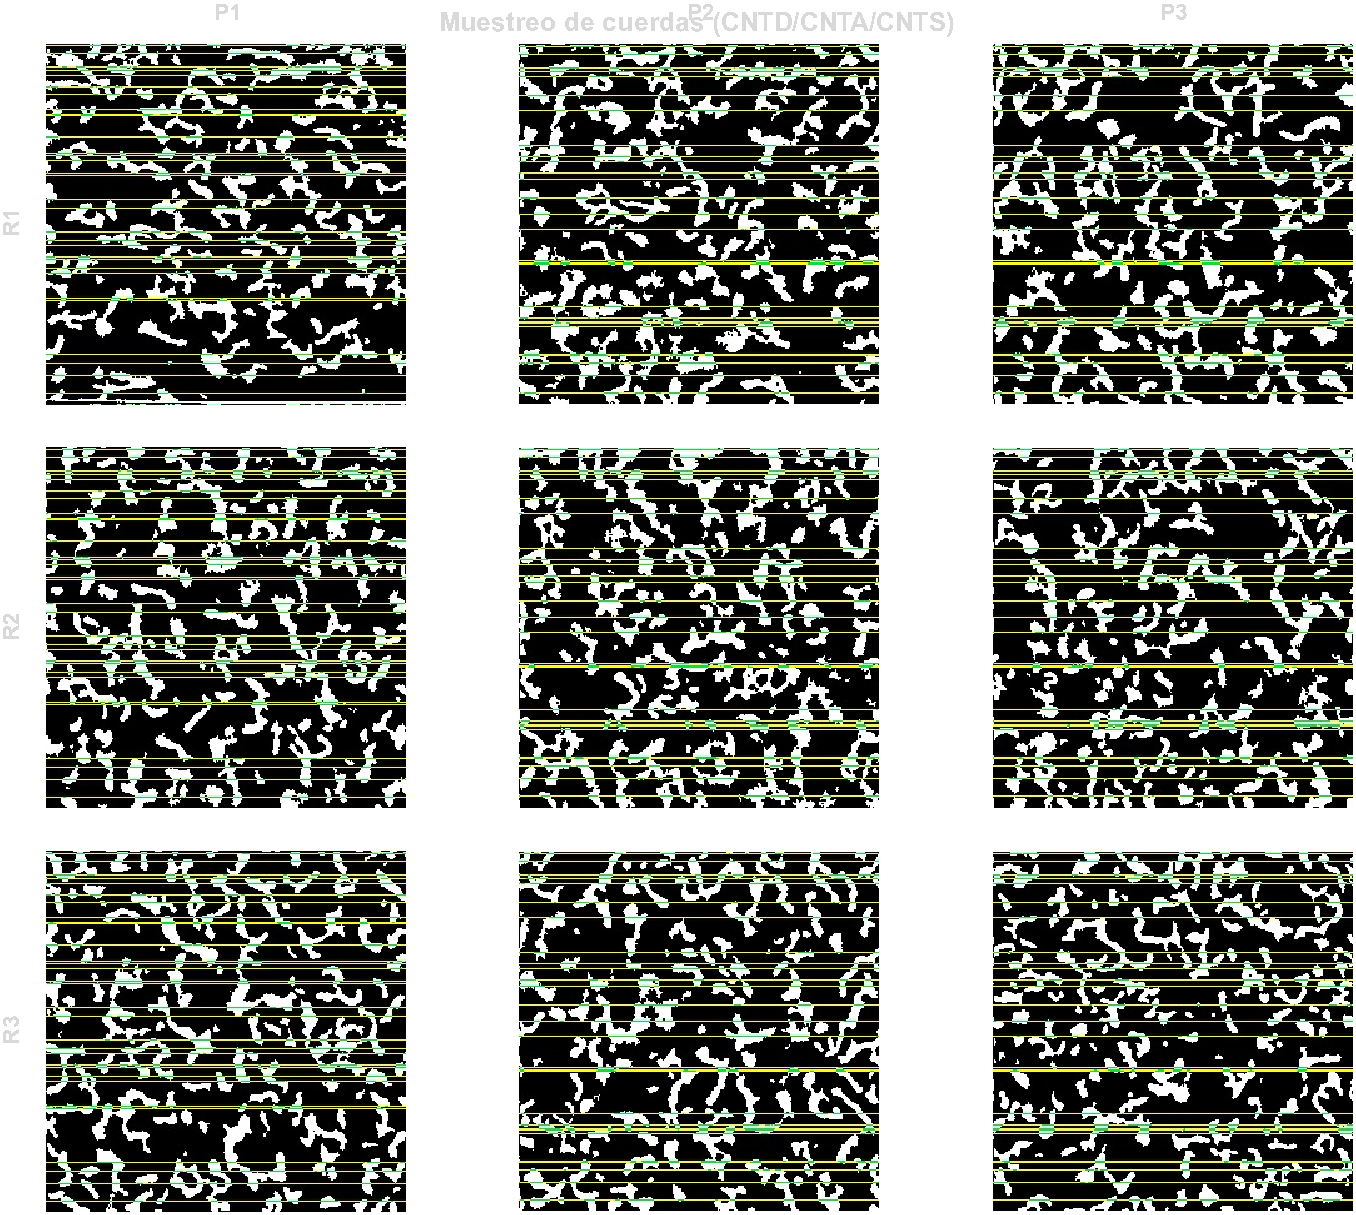
\includegraphics[width=0.6\textwidth]{mosaico_espacial.pdf}
    \caption{Muestreo de líneas para los descriptores de distribución espacial sobre el set 2b (15~V, 1~kHz; réplicas en filas, posiciones en columnas). Sobre la máscara morfológica $M_{\mathrm{C}}$ se trazan en amarillo las filas seleccionadas; los segmentos verdes marcan los tramos de CNT, cuyas longitudes alimentan CNTA, y los espacios entre ellos, los espaciados que alimentan CNTD.}
    \label{fig:met_espacial}
\end{figure}

\begingroup\color{red}
\subsubsection{Comparación de Binarizaciones para Reproducibilidad}
\label{sec:met_reproducibilidad}
\comentario{Revisando esta parte me di cuenta de que falta un espacio en la metodología para la validación de lo que se muestra en resultados, o al menos para declarar su alcance: la validación de parámetros, el análisis de robustez (cobertura, número de componentes y fragmentación normalizada, con su coeficiente de variación entre mediciones), la comparación con otros métodos de binarización y el comportamiento de los descriptores.}

Dado que CNTD, CNTA y CNTS se calculan a partir de una máscara binaria, su valor depende del método de binarización. Para evaluar si la dependencia de CNTS con el voltaje reportada en [4] se reproduce sobre este conjunto de datos, y si dicha reproducción depende del procesamiento propio, los tres descriptores se recalculan sobre las mismas mediciones con tres máscaras distintas. El procedimiento de cálculo de los descriptores y las 100 filas seleccionadas (misma semilla) son idénticos en los tres casos, de modo que la máscara es la única variable:

\begin{enumerate}
    \item \textbf{Procesamiento propio:} la máscara morfológica $M_{\mathrm{C}}$ de este trabajo.
    \item \textbf{Método de [4]:} sobre el canal eléctrico original $E_0$, escalado al intervalo $[0,1]$ entre su mínimo y su máximo (\texttt{mat2gray}), se aplican una ecualización adaptativa de histograma con limitación de contraste (CLAHE, función \texttt{adapthisteq} con sus parámetros por defecto), un filtro de mediana de $3\times3$ (\texttt{medfilt2}) y un umbral igual al 75~\% del valor máximo de la matriz resultante: los píxeles que lo superan toman el valor 1 y el resto el valor 0, tal como se describe en [4].
    \item \textbf{Umbral de [4] sobre el preprocesamiento propio:} el mismo procedimiento del punto anterior, sin la ecualización CLAHE, aplicado a $E_{\mathrm{seg}}$ en lugar de $E_0$. Con ello se aísla el efecto de la binarización, manteniendo fijo el preprocesamiento.
\end{enumerate}

Se compara CNTS en función del voltaje a 10~Hz, la única frecuencia comparable con [4], para las tres máscaras.
\endgroup


\subsection{Descriptores de Forma}

Estos descriptores caracterizan el tamaño y la forma de las regiones de la red, y cuánto se desvían sus estructuras de una trayectoria recta. Se calculan sobre las componentes conexas $C_k$ de $M_{\mathrm{C}}$ con la función \texttt{regionprops} de MATLAB [6], salvo la tortuosidad, que se calcula sobre el esqueleto $S$.

\paragraph{Área media y desviación estándar del área.}
El área de cada componente es su número de píxeles multiplicado por el área de un píxel, $A_k = |C_k|\,\Delta^2$, expresada en $\mu$m$^2$. Los descriptores son la media y la desviación estándar muestral de las áreas de las $N_{\mathrm{C}}$ componentes:

\begin{equation}
\bar A = \frac{1}{N_{\mathrm{C}}}\sum_{k=1}^{N_{\mathrm{C}}} A_k, \qquad
s_A = \sqrt{\frac{1}{N_{\mathrm{C}}-1}\sum_{k=1}^{N_{\mathrm{C}}} \left(A_k - \bar A\right)^2}
\label{eq:area}
\end{equation}

\paragraph{Elongación media.}
A cada componente se asocia la elipse que tiene sus mismos momentos centrales de segundo orden [6]; $a_k$ y $b_k$ son las longitudes de los ejes mayor y menor de esa elipse, en píxeles (parámetros \texttt{MajorAxisLength} y \texttt{MinorAxisLength} de \texttt{regionprops}). El descriptor es el promedio, sobre las $N_{\mathrm{C}}$ componentes, del cociente entre ambos ejes:

\begin{equation}
\bar e = \frac{1}{N_{\mathrm{C}}}\sum_{k=1}^{N_{\mathrm{C}}} \frac{a_k}{b_k}
\label{eq:elong}
\end{equation}

Un cociente igual a 1 corresponde a una componente sin dirección preferente, como un disco, y valores mayores, a componentes alargadas.

\paragraph{Tortuosidad media.}
La tortuosidad compara la longitud de una estructura medida a lo largo de su trayectoria con la distancia en línea recta entre sus extremos. Se calcula sobre las componentes conexas del esqueleto $S$, con vecindad de 8 píxeles. En cada componente se identifican sus puntos extremos, es decir, los píxeles con un único vecino de valor 1 (función \texttt{bwmorph} con la opción \texttt{'endpoints'}), y se mide la distancia geodésica entre ellos, definida como la longitud del camino más corto que los une recorriendo únicamente píxeles del esqueleto, con pasos de longitud 1 entre píxeles que comparten un lado y $\sqrt{2}$ entre píxeles que comparten una esquina (función \texttt{bwdistgeodesic} con la opción \texttt{'quasi-euclidean'}).

El par de extremos más alejados se identifica en dos pasos: primero se calcula la distancia geodésica desde un extremo cualquiera de la componente y se toma el extremo más lejano, $a$; después se calcula la distancia geodésica desde $a$ y se toma el extremo más lejano, $b$. Este procedimiento identifica el par de extremos con la mayor distancia geodésica cuando la componente no contiene ciclos. La longitud de arco de la componente es la distancia geodésica entre $a$ y $b$, $L^{(\text{arco})}$, y la cuerda es la distancia euclidiana entre ellos, $L^{(\text{cuerda})} = \sqrt{(x_a - x_b)^2 + (y_a - y_b)^2}$, ambas en píxeles. Solo se consideran las componentes con al menos 8 píxeles, al menos dos extremos y una longitud de arco de al menos 15 píxeles ($\approx 0.9$~$\mu$m), de modo que los fragmentos cortos, cuya tortuosidad es poco representativa, no intervienen. Si $M$ es el número de componentes que cumplen estas condiciones, el descriptor es

\begin{equation}
\bar\tau = \frac{1}{M}\sum_{m=1}^{M} \frac{L_m^{(\text{arco})}}{L_m^{(\text{cuerda})}}
\label{eq:tort}
\end{equation}

Cuantifica cuánto se desvían las estructuras de la red respecto de una trayectoria recta entre sus extremos: valores cercanos a 1 corresponden a estructuras casi rectas, y valores mayores, a estructuras más sinuosas.

\begin{figure}[H]
    \centering
    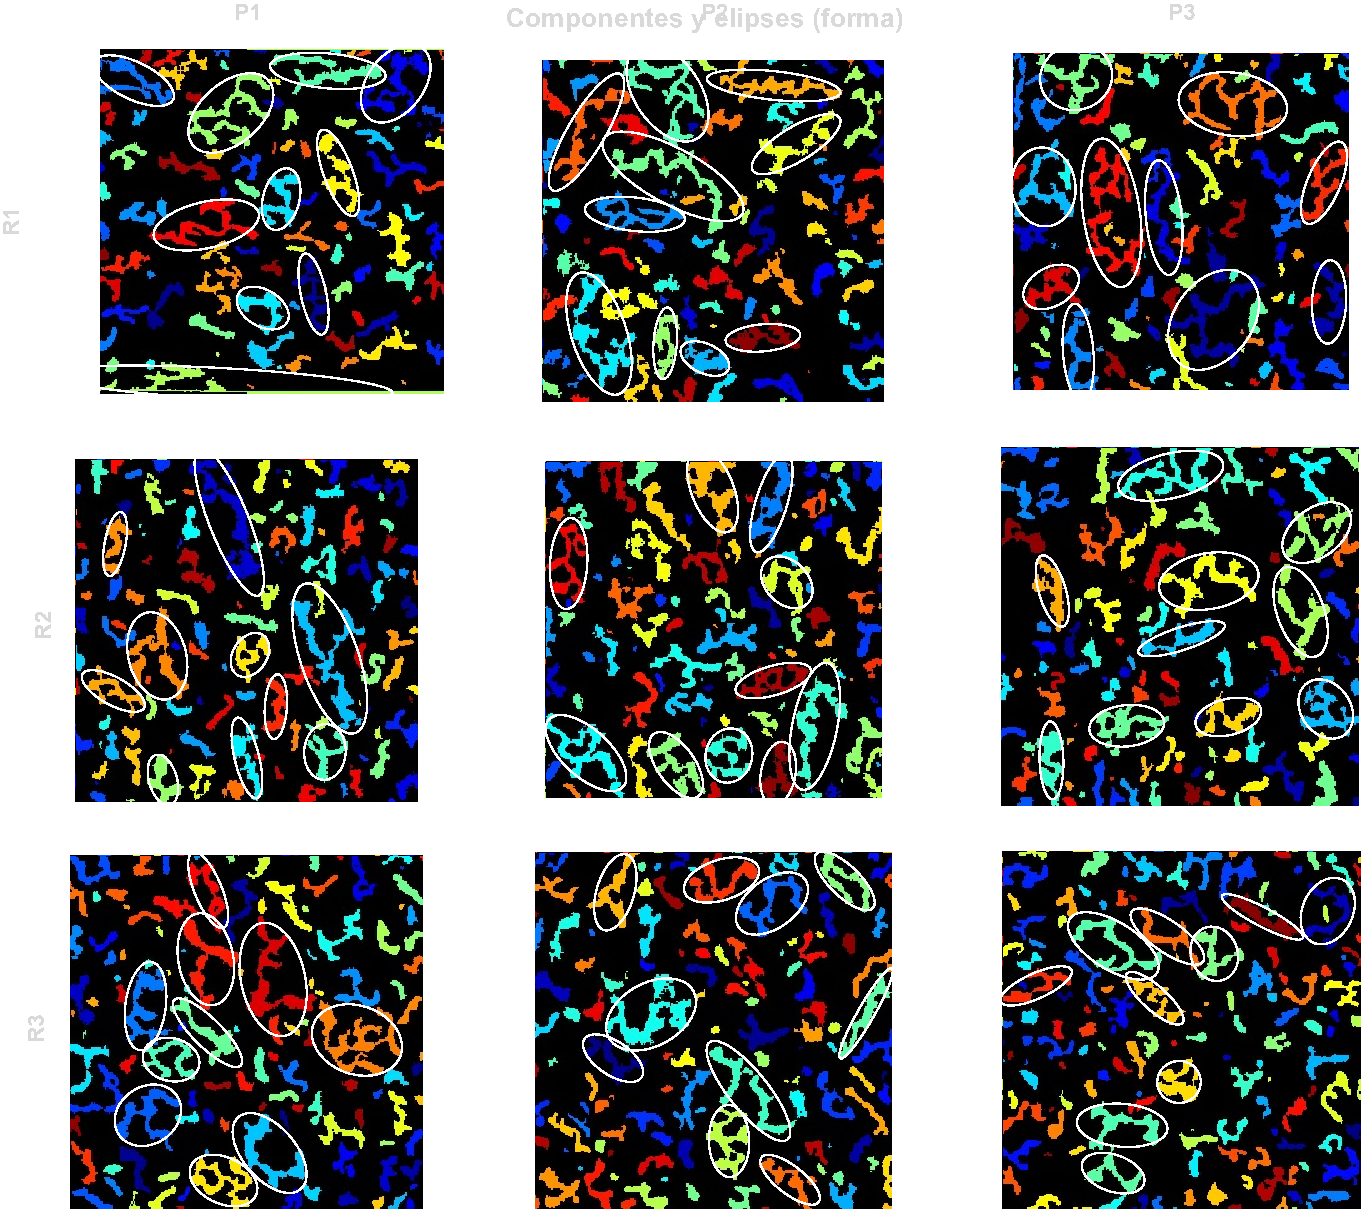
\includegraphics[width=0.6\textwidth]{mosaico_forma.pdf}
    \caption{Componentes conexas de la máscara morfológica $M_{\mathrm{C}}$ del set 2b, coloreadas por etiqueta, con las elipses de igual momento de segundo orden superpuestas sobre las mayores. Los ejes de cada elipse definen la elongación de la componente, y su número de píxeles, el área.}
    \label{fig:met_forma}
\end{figure}


\subsection{Descriptores de Orientación}

Estos descriptores cuantifican si las estructuras de la red siguen una dirección preferente. La orientación se evalúa mediante el tensor de estructura [6], calculado sobre la máscara morfológica $M_{\mathrm{C}}$. Como el gradiente de una máscara binaria solo es distinto de cero en los bordes y cambia de forma abrupta, la máscara se suaviza primero con un núcleo gaussiano de desviación estándar $\sigma_d = 2$~px, según (\ref{eq:gauss}), con la función \texttt{imgaussfilt}, lo que produce una matriz de valores continuos $Q = G_{\sigma_d} * M_{\mathrm{C}}$, donde $*$ denota la convolución. Sobre $Q$ se calculan las derivadas $\partial Q/\partial x$ y $\partial Q/\partial y$ por diferencias centrales, según (\ref{eq:diferencias}), y los productos de las derivadas se promedian localmente con un segundo núcleo gaussiano, de desviación estándar $\sigma_i = 8$~px:

\begin{equation}
J_{xx} = G_{\sigma_i} * \left(\frac{\partial Q}{\partial x}\right)^2, \qquad
J_{yy} = G_{\sigma_i} * \left(\frac{\partial Q}{\partial y}\right)^2, \qquad
J_{xy} = G_{\sigma_i} * \left(\frac{\partial Q}{\partial x}\,\frac{\partial Q}{\partial y}\right)
\label{eq:tensor_local}
\end{equation}

La escala $\sigma_d$ se ajusta al grosor de las estructuras de la red, y $\sigma_i$, a la escala sobre la que se promedia su dirección. Las tres componentes se suman sobre los píxeles de la red, es decir, sobre los píxeles de valor 1 de $M_{\mathrm{C}}$, y forman el tensor de estructura de la medición:

\begin{equation}
T =
\begin{pmatrix}
T_{xx} & T_{xy} \\
T_{xy} & T_{yy}
\end{pmatrix}, \qquad
T_{xx} = \sum_{M_{\mathrm{C}}(i,j) = 1} J_{xx}(i,j), \quad
T_{yy} = \sum_{M_{\mathrm{C}}(i,j) = 1} J_{yy}(i,j), \quad
T_{xy} = \sum_{M_{\mathrm{C}}(i,j) = 1} J_{xy}(i,j)
\label{eq:tensor}
\end{equation}

Los valores propios de $T$, $\xi_1 \ge \xi_2 \ge 0$, son

\begin{equation}
\xi_{1,2} = \frac{T_{xx} + T_{yy}}{2} \pm \frac{1}{2}\sqrt{(T_{xx} - T_{yy})^2 + 4T_{xy}^2}
\label{eq:valores_propios}
\end{equation}

El vector propio asociado a $\xi_1$ indica la dirección en que la intensidad de $Q$ varía más, que es perpendicular a las estructuras; la dirección de las estructuras es la perpendicular a esta. Los descriptores se calculan solo si $M_{\mathrm{C}}$ contiene más de 10 píxeles de valor 1 y $T_{xx} + T_{yy} > 0$.

\paragraph{Orientación dominante.}
Ángulo de la dirección de las estructuras, obtenido al sumar $90^\circ$ al ángulo del vector propio asociado a $\xi_1$ y expresado en el intervalo $[0^\circ, 180^\circ)$:

\begin{equation}
\theta_d = \left(\frac{1}{2}\,\mathrm{atan2}\left(2T_{xy},\; T_{xx} - T_{yy}\right) + 90^\circ\right) \bmod 180^\circ
\label{eq:orientacion}
\end{equation}

donde $\mathrm{atan2}(v, u)$ es el ángulo del vector $(u, v)$ respecto del eje $x$, en el intervalo $(-180^\circ, 180^\circ]$. El ángulo se mide desde el eje $x$, es decir, desde la dirección de la línea de barrido, hacia el sentido creciente del índice de fila $i$; como las filas crecen hacia abajo en la imagen, el ángulo crece en sentido horario sobre la imagen.

\paragraph{Coherencia.}
Relación entre la diferencia y la suma de los valores propios:

\begin{equation}
\kappa = \frac{\xi_1 - \xi_2}{\xi_1 + \xi_2}
\label{eq:coherencia}
\end{equation}

Valores próximos a 1 indican una alta alineación direccional, y valores próximos a 0, una red isótropa. La coherencia delimita además la validez de la orientación dominante: en una red casi isótropa no existe una dirección preferente bien definida, por lo que $\theta_d$ solo es significativa cuando $\kappa$ es apreciable.

\begin{figure}[H]
    \centering
    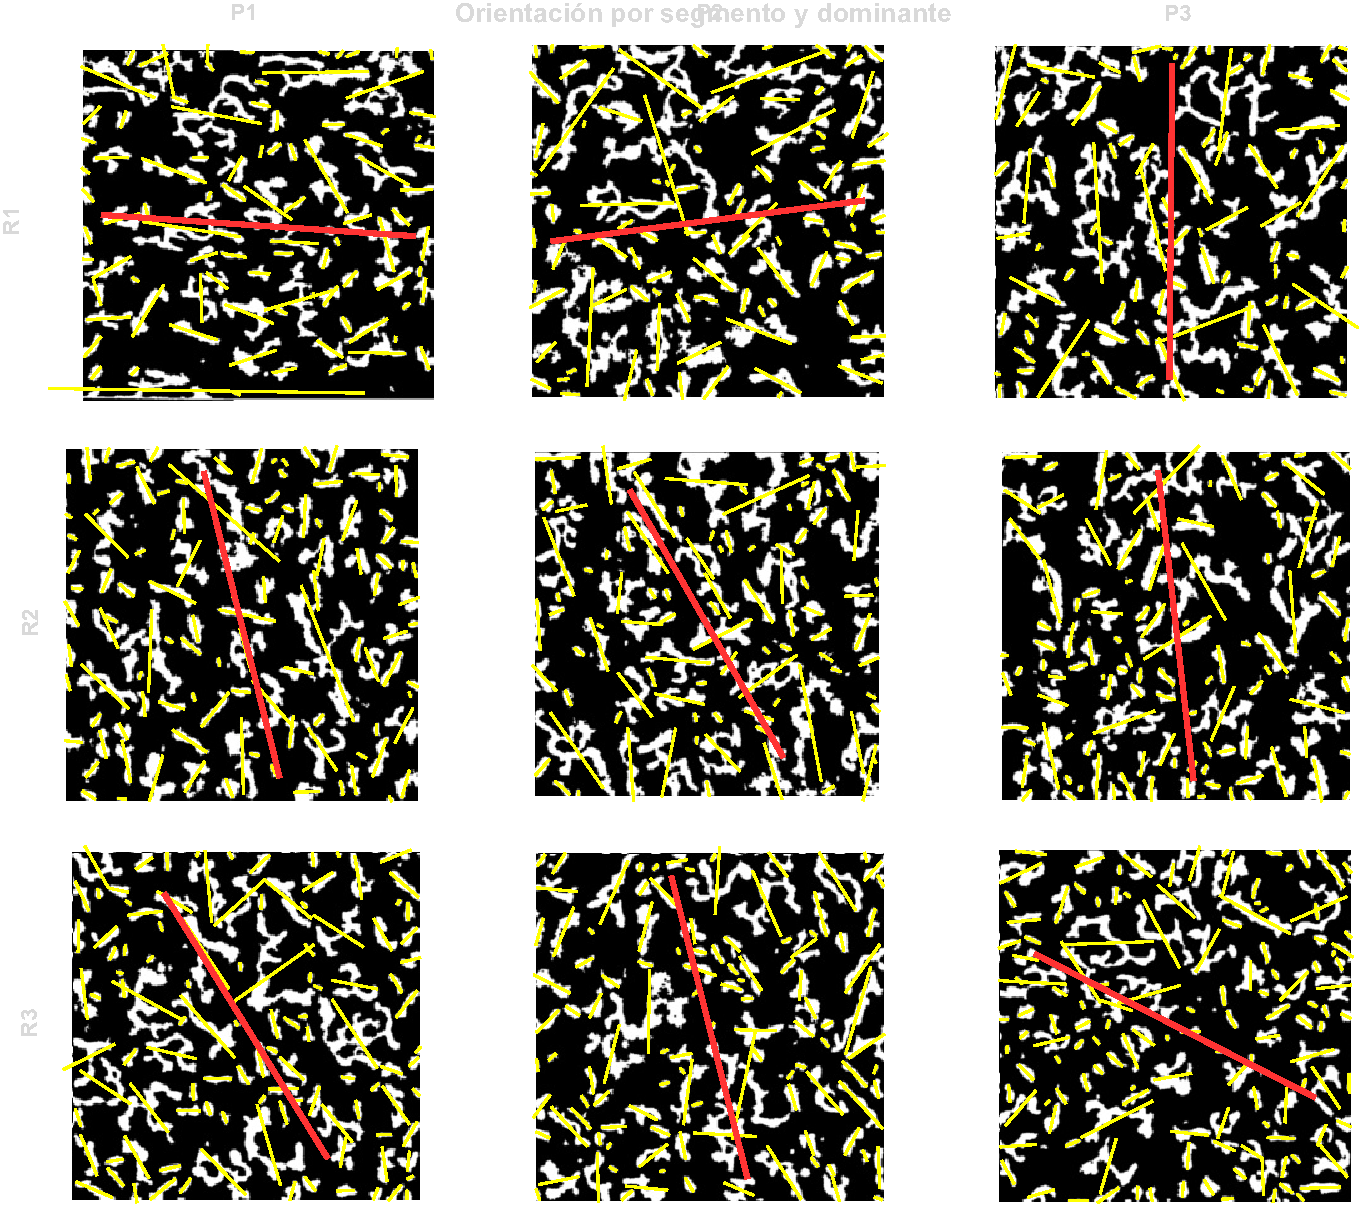
\includegraphics[width=0.6\textwidth]{mosaico_orientacion.pdf}
    \caption{Orientación de la red para las nueve mediciones del set 2b. Cada barra amarilla indica la orientación de una componente de $M_{\mathrm{C}}$, obtenida con el tensor de estructura sumado sobre los píxeles de esa componente, y la barra roja marca la orientación dominante $\theta_d$ de la medición.}
    \label{fig:met_orientacion}
\end{figure}


\subsection{Descriptores de Conectividad y Topología}

Estos descriptores evalúan la red como un todo: qué fracción de la superficie ocupa, en qué medida forma una estructura continua y cuán extensa es.

\paragraph{Cobertura total.}
Fracción de píxeles clasificados como red, $c(M_{\mathrm{F}})$, definida en (\ref{eq:cobertura}). Se calcula sobre la máscara final y no sobre $M_{\mathrm{C}}$, para no incluir los píxeles que agrega el cierre morfológico.

\paragraph{Índice de percolación.}
Cociente entre el área de la componente conexa más grande de $M_{\mathrm{C}}$ y el área total ocupada por todas las componentes:

\begin{equation}
P_{\mathrm{perc}} = \frac{\max_k |C_k|}{\sum_{k=1}^{N_{\mathrm{C}}} |C_k|}
\label{eq:percolacion}
\end{equation}

Cuantifica la dominancia de la componente mayor sobre la red segmentada: valores cercanos a 1 indican que casi toda la red pertenece a una sola estructura conexa. El índice no evalúa si esa componente atraviesa la medición de un borde a otro.

\paragraph{Longitud de red.}
Longitud total del esqueleto $S$, obtenida al sumar las distancias entre sus píxeles vecinos:

\begin{equation}
L_S = \left(n_o + \sqrt{2}\, n_d\right) \Delta
\label{eq:longitud}
\end{equation}

donde $n_o$ es el número de pares de píxeles de valor 1 de $S$ que comparten un lado, y $n_d$, el número de pares que comparten solo una esquina y cuyos dos vecinos comunes tienen valor 0. Esta condición evita contar dos veces un mismo recorrido: si dos píxeles diagonales están unidos también a través de un vecino común, el recorrido ya está contado por los pasos horizontal y vertical. $L_S$ se expresa en $\mu$m.

\paragraph{Número de fragmentos.}
Número de componentes conexas de $M_{\mathrm{C}}$, $N_{\mathrm{C}}$, calculado con la función \texttt{bwconncomp} con vecindad de 8 píxeles. Un número alto indica una red dividida en muchas regiones aisladas.

\begin{figure}[H]
    \centering
    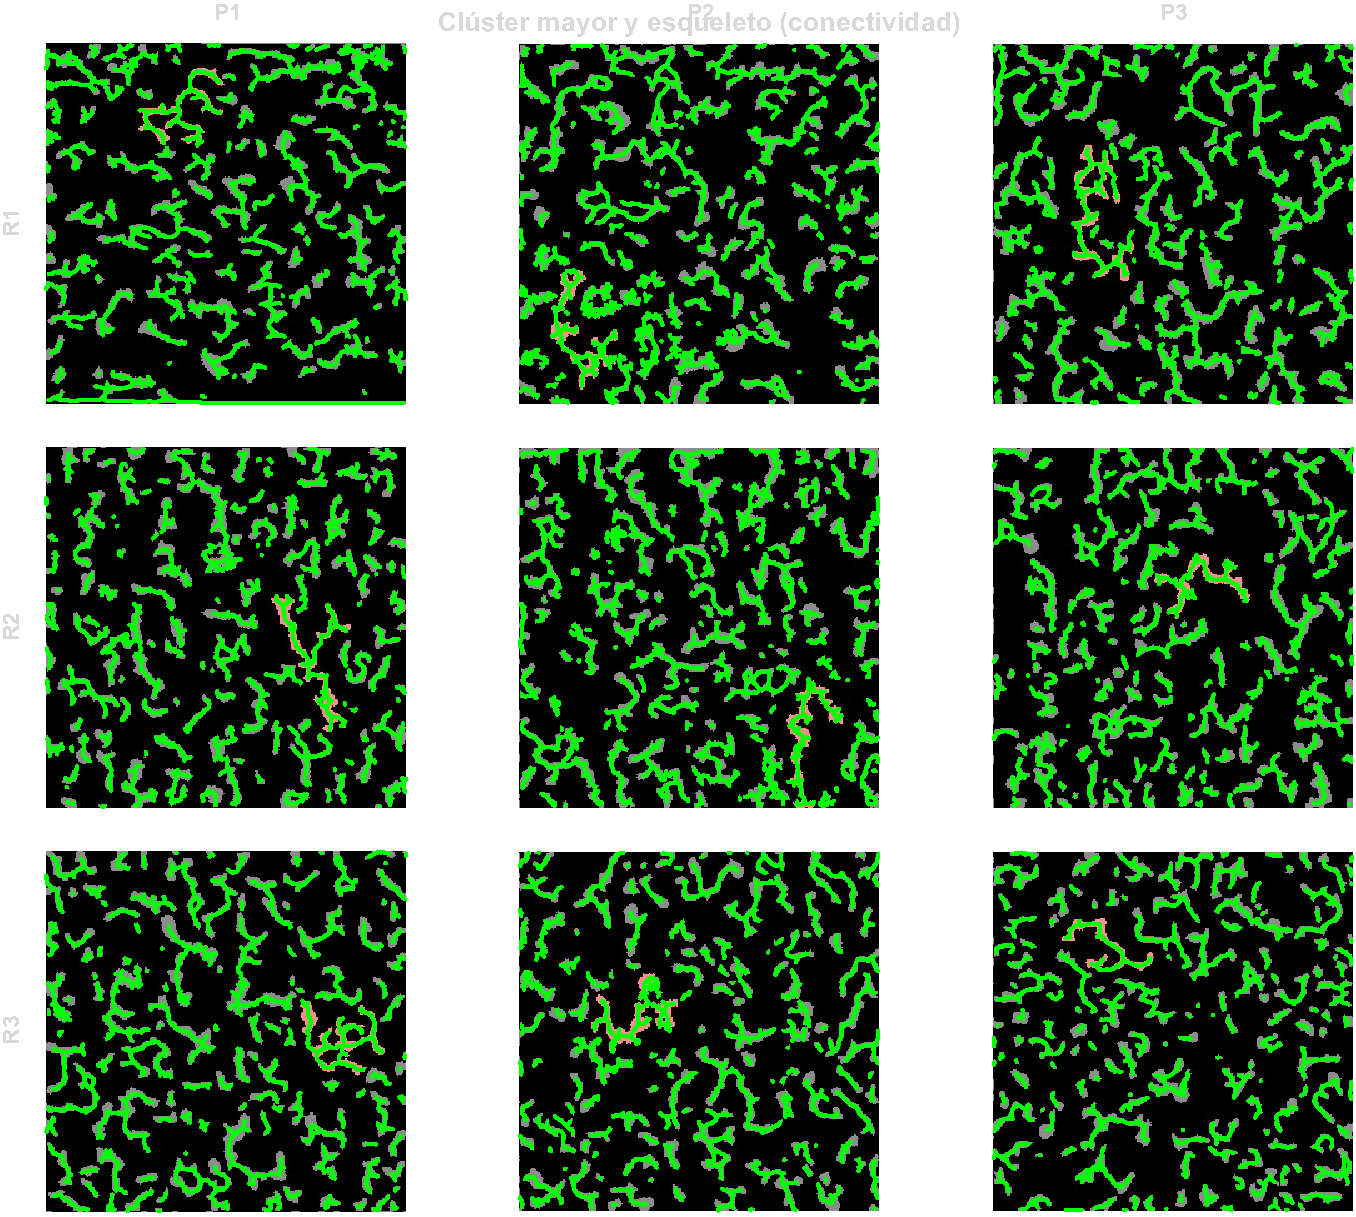
\includegraphics[width=0.6\textwidth]{mosaico_conectividad.pdf}
    \caption{Análisis de conectividad sobre el set 2b: la componente conexa de mayor área de $M_{\mathrm{C}}$ se resalta en rojo (base del índice de percolación) y el esqueleto $S$ se superpone en verde (base de la longitud de red).}
    \label{fig:met_conectividad}
\end{figure}


\section{Análisis de Datos y Aprendizaje Automático}
\label{sec:met_analisis}
 
A partir de los 13 descriptores extraídos por medición se construye la matriz de
descriptores $X$, de $81 \times 13$, que constituye el insumo del análisis. Este se organiza en dos
etapas. La primera es un análisis exploratorio no supervisado que caracteriza la estructura interna del espacio de descriptores y su redundancia. La segunda corresponde a los modelos supervisados:
el análisis predictivo de regresión hacia la eficacia de apantallamiento (SE),
que constituye el objetivo central del trabajo.
 
\subsection{Análisis Exploratorio de Descriptores}
\label{sec:met_exploratorio}
 
Cada descriptor genera una distribución de 81 valores sobre el dataset. Sobre la
matriz estandarizada (media cero, varianza unitaria) se aplican dos
herramientas complementarias.
 
\paragraph{Estructura de correlación.} Se calcula la matriz de correlación de
Pearson entre los 13 descriptores. Para identificar grupos de descriptores
redundantes se aplica un agrupamiento jerárquico de enlace promedio sobre la
distancia $d_{ij}=1-|r_{ij}|$, que une descriptores fuertemente correlacionados
(en cualquier signo) en familias.
 
\paragraph{Dimensionalidad efectiva.} Mediante análisis de componentes
principales (PCA) se cuantifica la dimensionalidad real del espacio. Se reporta
la varianza explicada acumulada y la dimensionalidad efectiva mediante el
\textit{participation ratio} $\mathrm{PR}=\left(\sum_i \lambda_i\right)^2 / \sum_i \lambda_i^2$,
donde $\lambda_i$ son los valores propios de la matriz de covarianza. PR estima
el número de direcciones que concentran la varianza con independencia de cuántos
descriptores se midan.

\begin{comment}
\section{Machine Learning}
A partir de los datos de fabricación, mediciones de descriptores y valores de SE, se construyen los datos que se van a usar en los diferentes procesos de Machine Learning.

\subsection{Dataset ML}
\subsubsection{Datos para Regresión}
Este análisis se realiza sobre la unidad de medición de las propiedades de SE. Estas mediciones generalmente pueden hacerse de la siguiente forma:
\begin{itemize}
    \item Medición de SE por grupo de fabricación (9 Datos).
\item Medición de SE por Réplica  (27 Datos).
\item Medición de SE por Muestra (81 Datos).
\end{itemize}
Dependiendo de esta magnitud se deben hacer transformaciones en el dataset los descriptores medidos, puesto que en ese caso si se realiza una extracción de descriptores a cada imagen (81 datos por cada descriptor). En caso de que los valores de SE sean por réplica  o por grupo de fabricación, se harán simplificaciones en los subconjuntos, tomando valores representativos de los mismos; como por ejemplo la mediana de cada descriptor para igualar el número de datos de SE y eliminar problemas de dependencia.

Al momento no se ha desarrollado, así que este análisis queda planteado, pero sigue como trabajo en progreso.

\subsubsection{Datos para Clasificación}
Se obtendrán 20 descriptores, junto a los datos de las características de fabricación, extraídos individualmente de las 81 imágenes. Esto nos deja con un problema de clasificación de 9 clases Voltaje-Frecuencia. Las 81 imágenes no son estadísticamente independientes entre sí, dado que las tres imágenes de una misma réplica provienen del mismo espécimen físico. Por ello, para evitar problemas con la asignación aleatoria de las imágenes en el modelo, que puedan llevar a la separación de muestras de una misma réplica, se usara GroupKFold, asegurando que permanezcan en conjunto. Finalmente se aclara la ejecución de estandarización de las variables.

\subsection{Pipeline de Clasificación Exploratoria}
Su implementación se realiza en Matlab y comprende GroupKFold, los modelos, métricas de evaluación y Análisis de interpretabilidad.

\subsubsection{Estrategia de Validación}
 La validación cruzada se realiza mediante GroupKFold agrupando por réplica. El dataset cuenta con 27 réplicas (3 réplicas × 9 condiciones) que se distribuyen en K = 3 folds, asignando 9 réplicas a cada fold. En cada iteración, dos folds (54 imágenes correspondientes a 18 réplicas) se utilizan para entrenamiento y un fold (27 imágenes correspondientes a 9 réplicas) para prueba. Las métricas reportadas corresponden al promedio sobre los tres folds.

 Para el desempeño del modelo se usan las siguientes métricas:

 \begin{itemize}
     \item Accuracy: Porcentaje de imágenes correctamente clasificadas.
     \item F1 Macro: Media armónica de precisión y recall, promediada por clase sin ponderar. Permite detectar si el modelo tiene desempeño desigual entre clases.
     \item Matriz de Confusión: Representación visual de aciertos y errores entre cada par de clases. Su utilidad en este análisis es identificar qué condiciones V×f resultan más confundibles entre si.
 \end{itemize}

 \subsubsection{Modelos}
 Para el análisis clasificatorio se desarrollan los siguientes modelos: Random Forest Classifier y Análisis Discriminante Lineal (LDA). En este caso, y al ser un análisis exploratorio, se establecen los parámetros por defecto de Matlab en los modelos. Esto derivado del reducido tamaño del dataset, y de no tener la intención de producir un sistema predictivo ideal, sino de simplemente analizar cómo se comportan los descriptores frente a los parámetros de fabricación.

 Para Random Forest se utiliza la función TreeBagger de MATLAB con 100 árboles, valor que ofrece estabilidad estadística sin coste computacional excesivo en datasets pequeños. LDA se entrena directamente con fitcdiscr sin parámetros especiales, dado que el método tiene formulación cerrada y no requiere tuning relevante.
 
 \subsubsection{Interpretabilidad}
 La interpretabilidad del modelo frente a los descriptores esta dada por diferentes métricas:
 
 Importancia de variables del Random Forest: Cada árbol del bosque contribuye con una medida de cuánto reduce cada descriptor el error de clasificación a lo largo de los splits en los que se utiliza. La importancia agregada del bosque se calcula promediando estas contribuciones sobre los 100 árboles.

 Importancia por permutación: Para cada descriptor, se mide la pérdida de exactitud del modelo cuando los valores de ese descriptor se permutan aleatoriamente entre las observaciones del fold de prueba. Una caída grande indica que el descriptor era relevante; una caída nula indica que el modelo no dependía de él [7]. Esta medida es agnóstica al tipo de modelo y se aplica tanto a Random Forest como a LDA, permitiendo comparar la importancia atribuida a cada descriptor por modelos de naturalezas distintas.

 Coeficientes lineales del LDA: La matriz de proyección del LDA asigna pesos a cada descriptor para construir las direcciones de máxima separación entre clases. Aunque el LDA proyecta sobre múltiples direcciones discriminantes, la primera dirección (asociada al mayor valor propio) concentra la información de mayor varianza entre clases y permite identificar qué descriptores dominan dicha separación.

 Los rankings de importancia obtenidos por estas tres rutas se contrastarán entre sí. La concordancia entre ellos es indicio de relevancia robusta de un descriptor; la divergencia indica que el papel de ese descriptor depende del tipo de modelo y debe interpretarse con cuidado.
 
\end{comment}


\chapter{Resultados}

Este capítulo presenta los hallazgos obtenidos al aplicar la metodología descrita en el capítulo anterior al conjunto de 81 imágenes del gradiente de capacitancia. La estructura sigue el orden metodológico, separando los hallazgos asociados al procesamiento digital de imágenes y a la extracción de descriptores morfológicos correspondientes a los primeros objetivos específicos.

A lo largo del capítulo se utilizan dos niveles de evidencia complementarios. Por un lado, se reportan estadísticos por imagen para el set de fabricación 2b (15~V, 1~kHz), seleccionado como referencia visual por su uniformidad y consistencia entre las nueve mediciones, junto con los resúmenes estadísticos del propio set y del conjunto global de 81 imágenes (media, desviación estándar, mínimo, mediana y máximo). Por otro, se muestran mosaicos $3\times3$ de las 9 imágenes del set 2b en cada etapa del pipeline (réplicas en filas, posiciones en columnas), que permiten contrastar visualmente el efecto de cada operación.

\section{Procesamiento Digital de Imágenes}

\subsection{Corrección de Crosstalk Topográfico}

La Tabla~\ref{tab:crosstalk_2b} reporta la correlación de Pearson entre la señal eléctrica y la topográfica antes de la corrección, para las 9 imágenes del set 2b, junto con los resúmenes estadísticos del set y del conjunto global. La correlación residual posterior a la corrección no se incluye en la tabla, ya que es del orden de $10^{-16}$ por construcción del ajuste por mínimos cuadrados.

\begin{figure}[H]
\centering
\begin{minipage}[t]{0.42\textwidth}
\centering
\vspace{0pt}
\includegraphics[width=\textwidth]{01_raw_2b.pdf}\\[2pt]
\includegraphics[width=\textwidth]{02_crosstalk_2b.pdf}
\caption{Mosaicos $3\times3$ del set 2b antes (arriba) y después (abajo) de la corrección de crosstalk topográfico.}
\label{fig:res_crosstalk}
\end{minipage}\hfill
\begin{minipage}[t]{0.55\textwidth}
\centering
\vspace{0pt}
\captionof{table}{Correlación lineal entre la señal eléctrica cruda y la topográfica antes de la corrección de crosstalk.}
\label{tab:crosstalk_2b}
\small
\begin{tabular}{lc}
\toprule
\textbf{Imagen / Estad.} & \textbf{Corr. pre-filtro} \\
\midrule
2b-1 & $\phantom{-}0.0522$ \\
2b-2 & $\phantom{-}0.0040$ \\
2b-3 & $-0.0121$ \\
2b-4 & $\phantom{-}0.0212$ \\
2b-5 & $\phantom{-}0.1230$ \\
2b-6 & $-0.0062$ \\
2b-7 & $\phantom{-}0.0331$ \\
2b-8 & $-0.1085$ \\
2b-9 & $-0.0226$ \\
\midrule
\multicolumn{2}{l}{\textit{Resumen Set 2b}} \\
\quad Media           & $\phantom{-}0.0093$ \\
\quad Desv. estándar  & $\phantom{-}0.0623$ \\
\quad Mínimo          & $-0.1085$ \\
\quad Mediana         & $\phantom{-}0.0040$ \\
\quad Máximo          & $\phantom{-}0.1230$ \\
\midrule
\multicolumn{2}{l}{\textit{Resumen Global ($n=81$)}} \\
\quad Media           & $-0.0285$ \\
\quad Desv. estándar  & $\phantom{-}0.0750$ \\
\quad Mínimo          & $-0.2125$ \\
\quad Mediana         & $-0.0134$ \\
\quad Máximo          & $\phantom{-}0.1332$ \\
\bottomrule
\end{tabular}
\end{minipage}
\end{figure}

A nivel global, los valores individuales de correlación pre-filtro alcanzan extremos de $-0.2125$ y $0.1332$ a lo largo del dataset. Tras la aplicación del modelo, la correlación residual se anula a nivel numérico para todas las imágenes del conjunto.


\subsection{Filtrado de Ruido Impulsivo}

La Tabla~\ref{tab:impulsivo_2b} reporta el porcentaje de píxeles reemplazados por las dos instancias del filtro: la primera, aplicada tras la corrección de crosstalk con kernel $5\times5$ y umbral $3\sigma$ para suprimir ruido sal y pimienta; la segunda, aplicada tras la corrección de fondo con kernel $5\times1$ y umbral $2\sigma$ para suprimir líneas impulsivas horizontales.

\begin{figure}[H]
\centering
\begin{minipage}[t]{0.48\textwidth}
\centering
\vspace{0pt}
\includegraphics[width=\textwidth]{03_syp5x5_2b.pdf}\\[2pt]
\includegraphics[width=\textwidth]{05_syp5x1_2b.pdf}
\caption{Mosaicos $3\times3$ del set 2b tras las dos instancias del filtro. Arriba: tras SyP $5\times5$. Abajo: tras filtro de líneas $5\times1$.}
\end{minipage}\hfill
\begin{minipage}[t]{0.49\textwidth}
\centering
\vspace{0pt}
\captionof{table}{Porcentaje de píxeles reemplazados por las dos instancias del filtro de ruido impulsivo.}
\label{tab:impulsivo_2b}
\small
\begin{tabular}{lcc}
\toprule
\textbf{Imagen / Estad.} & \textbf{SyP $5\times5$ [\%]} & \textbf{Líneas $5\times1$ [\%]} \\
\midrule
2b-1 & $4.35$ & $16.62$ \\
2b-2 & $1.57$ & $20.82$ \\
2b-3 & $0.49$ & $17.30$ \\
2b-4 & $0.31$ & $27.25$ \\
2b-5 & $0.44$ & $16.66$ \\
2b-6 & $0.40$ & $37.12$ \\
2b-7 & $1.07$ & $17.39$ \\
2b-8 & $1.48$ & $16.54$ \\
2b-9 & $0.68$ & $35.04$ \\
\midrule
\multicolumn{3}{l}{\textit{Resumen Set 2b}} \\
\quad Media           & $1.20$  & $22.75$ \\
\quad Desv. estándar  & $1.27$  & $\phantom{0}8.32$ \\
\quad Mínimo          & $0.31$  & $16.54$ \\
\quad Mediana         & $0.68$  & $17.39$ \\
\quad Máximo          & $4.35$  & $37.12$ \\
\midrule
\multicolumn{3}{l}{\textit{Resumen Global ($n=81$)}} \\
\quad Media           & $\phantom{0}3.73$ & $23.18$ \\
\quad Desv. estándar  & $\phantom{0}8.36$ & $\phantom{0}8.09$ \\
\quad Mínimo          & $\phantom{0}0.24$ & $14.26$ \\
\quad Mediana         & $\phantom{0}1.37$ & $19.60$ \\
\quad Máximo          & $47.32$           & $46.44$ \\
\bottomrule
\end{tabular}
\label{fig:res_impulsivo}
\end{minipage}
\end{figure}

La primera instancia reemplaza en promedio el 3.73\% de los píxeles a nivel global, con un máximo individual del 47.32\% sobre el conjunto completo. La segunda instancia reemplaza en promedio el 23.18\% global, con un mínimo del 14.26\% y un máximo del 46.44\%.


\subsection{Corrección de Artefactos de Barrido}

La Tabla~\ref{tab:artefactos_2b} reporta la varianza entre filas, calculada como la varianza de las medias por fila de la imagen, antes y después del ajuste descrito en la metodología.

\begin{figure}[H]
\centering
\begin{minipage}[t]{0.48\textwidth}
\centering
\vspace{0pt}
\includegraphics[width=\textwidth]{04_artefactos_2b.pdf}
\caption{Mosaico $3\times3$ del set 2b tras la corrección de artefactos de barrido.}
\label{fig:res_artefactos}
\end{minipage}\hfill
\begin{minipage}[t]{0.49\textwidth}
\centering
\vspace{0pt}
\captionof{table}{Varianza entre filas antes y después de la corrección de artefactos de barrido.}
\label{tab:artefactos_2b}
\small
\begin{tabular}{lcc}
\toprule
\textbf{Imagen / Estad.} & \textbf{Pre-filtro} & \textbf{Post-filtro} \\
\midrule
2b-1 & $2.5357$ & $0.5440$ \\
2b-2 & $3.6080$ & $0.0833$ \\
2b-3 & $1.5582$ & $0.0862$ \\
2b-4 & $1.7520$ & $0.0316$ \\
2b-5 & $0.4934$ & $0.0915$ \\
2b-6 & $0.7136$ & $0.1753$ \\
2b-7 & $0.8245$ & $0.3114$ \\
2b-8 & $0.9550$ & $0.2137$ \\
2b-9 & $0.3977$ & $0.2134$ \\
\midrule
\multicolumn{3}{l}{\textit{Resumen Set 2b}} \\
\quad Media           & $1.4265$  & $0.1945$ \\
\quad Desv. estándar  & $1.0686$  & $0.1574$ \\
\quad Mínimo          & $0.3977$  & $0.0316$ \\
\quad Mediana         & $0.9550$  & $0.1753$ \\
\quad Máximo          & $3.6080$  & $0.5440$ \\
\midrule
\multicolumn{3}{l}{\textit{Resumen Global ($n=81$)}} \\
\quad Media           & $\phantom{0}1.7284$  & $0.1313$ \\
\quad Desv. estándar  & $\phantom{0}2.0774$  & $0.1566$ \\
\quad Mínimo          & $\phantom{0}0.1920$  & $0.0086$ \\
\quad Mediana         & $\phantom{0}1.2605$  & $0.0862$ \\
\quad Máximo          & $16.3627$            & $1.1876$ \\
\bottomrule
\end{tabular}
\end{minipage}
\end{figure}

A nivel global, la media de la varianza entre filas se reduce de $1.7284$ a $0.1313$, una reducción superior a un orden de magnitud. La mediana sigue el mismo patrón ($1.2605 \to 0.0862$). El máximo individual pre-filtro ($16.36$) corresponde a una imagen con artefactos de escaneo extremos; tras el filtro su contribución se reduce a $1.1876$. La inspección visual de los mosaicos confirma el aplanamiento del fondo y la atenuación de los artefactos horizontales en todas las imágenes del conjunto.




\subsection{Segmentación Multiescala y Binarización}
 
La etapa final del procesamiento aísla la red de CNTs en máscaras binarias mediante la integración de tres binarizaciones complementarias. La configuración del pipeline (sensibilidad $0.55$, ventana local $21$~px, ventana regional $51$~px, $6$ clases en Otsu, $50$ píxeles mínimos por componente) se determinó por inspección visual durante el desarrollo, ajustando los parámetros hasta que las máscaras representaran adecuadamente la red sobre el conjunto de imágenes. Los mosaicos del set 2b en las salidas individuales de las tres binarizaciones se reportan en la Figura~\ref{fig:res_bin_individuales}.


 
\begin{figure}[H]
    \centering
    \begin{minipage}{0.48\textwidth}
        \centering
        \includegraphics[width=\textwidth]{06_norm_2b.pdf}
     
    \end{minipage}\hfill
    \begin{minipage}{0.48\textwidth}
        \centering
        \includegraphics[width=\textwidth]{07_bw_local_2b.pdf}
    \end{minipage}
 

 
    \begin{minipage}{0.48\textwidth}
        \centering
        \includegraphics[width=\textwidth]{08_bw_global_2b.pdf}
      
    \end{minipage}\hfill
    \begin{minipage}{0.48\textwidth}
        \centering
        \includegraphics[width=\textwidth]{09_bw_regional_2b.pdf}
      
    \end{minipage}
    \caption{Mosaicos $3\times3$ del set 2b en la etapa de binarización multiescala: señal normalizada de entrada y salidas individuales de las tres binarizaciones complementarias antes de la conjunción.}
    \label{fig:res_bin_individuales}
\end{figure}
 
La binarización local recupera estructuras de alta definición pero introduce fragmentación granular en regiones de fondo. La binarización global produce regiones de mayor extensión espacial con menor definición de borde. La binarización regional opera como filtro espacial de escala intermedia. La conjunción lógica de las tres máscaras y el cierre morfológico posterior dan lugar a las representaciones empleadas en la extracción de descriptores; sus mosaicos se reportan en la Figura~\ref{fig:res_bin_postproc}.
 
\begin{figure}[H]
\centering
\begin{minipage}[t]{0.3\textwidth}
\centering
\vspace{0pt}
\includegraphics[width=\textwidth]{10_bw2_2b.pdf}\\[2pt]
\includegraphics[width=\textwidth]{11_bw2closed_2b.pdf}\\[2pt]
\includegraphics[width=\textwidth]{12_skel_2b.pdf}
\caption{Mosaicos $3\times3$ del set 2b tras la integración. Arriba: máscara estricta $M_{\mathrm{F}}$. Centro: máscara morfológica $M_{\mathrm{C}}$. Abajo: esqueleto.}
\label{fig:res_bin_postproc}

\end{minipage}\hfill
\begin{minipage}[t]{0.7\textwidth}
\centering
\vspace{0pt}
\captionof{table}{Estadísticos por imagen sobre las máscaras y el esqueleto para el set 2b.}
\label{tab:bin_2b}
\footnotesize
\begin{tabular}{lccccc}
\toprule
\textbf{Imagen / Estad.} & \textbf{Cob. $M_{\mathrm{F}}$} & \textbf{$N_{c}$ $M_{\mathrm{F}}$} & \textbf{Cob. $M_{\mathrm{C}}$} & \textbf{$N_{c}$ $M_{\mathrm{C}}$} & \textbf{Skel [px]} \\
\midrule
2b-1 & $0.2005$ & $132$ & $0.2304$ & $\phantom{0}99$ & $12\,634$ \\
2b-2 & $0.2120$ & $155$ & $0.2531$ & $107$ & $13\,767$ \\
2b-3 & $0.2097$ & $128$ & $0.2465$ & $100$ & $12\,318$ \\
2b-4 & $0.2089$ & $162$ & $0.2396$ & $126$ & $11\,628$ \\
2b-5 & $0.2215$ & $161$ & $0.2649$ & $110$ & $13\,863$ \\
2b-6 & $0.2103$ & $154$ & $0.2370$ & $119$ & $11\,656$ \\
2b-7 & $0.2232$ & $150$ & $0.2522$ & $118$ & $11\,809$ \\
2b-8 & $0.2156$ & $150$ & $0.2457$ & $124$ & $11\,574$ \\
2b-9 & $0.2167$ & $169$ & $0.2305$ & $147$ & $10\,479$ \\
\midrule
\multicolumn{6}{l}{\textit{Resumen Set 2b}} \\
\quad Media           & $0.2132$ & $151.2$ & $0.2444$ & $116.7$ & $12\,192$ \\
\quad Desv. estándar  & $0.0070$ & $\phantom{0}13.5$  & $0.0114$ & $\phantom{0}15.0$  & $\phantom{0\,}1\,093$ \\
\quad Mínimo          & $0.2005$ & $128$   & $0.2304$ & $\phantom{0}99$    & $10\,479$ \\
\quad Mediana         & $0.2120$ & $154$   & $0.2457$ & $118$              & $11\,809$ \\
\quad Máximo          & $0.2232$ & $169$   & $0.2649$ & $147$              & $13\,863$ \\
\midrule
\multicolumn{6}{l}{\textit{Resumen Global ($n=81$)}} \\
\quad Media           & $0.2202$ & $180.6$ & $0.2597$ & $120.5$ & $14\,252$ \\
\quad Desv. estándar  & $0.0155$ & $\phantom{0}52.7$  & $0.0391$ & $\phantom{0}23.1$  & $\phantom{0\,}4\,651$ \\
\quad Mínimo          & $0.1811$ & $109$   & $0.1878$ & $\phantom{0}76$    & $\phantom{0\,}8\,045$ \\
\quad Mediana         & $0.2208$ & $162$   & $0.2529$ & $120$              & $13\,112$ \\
\quad Máximo          & $0.2749$ & $396$   & $0.4102$ & $217$              & $32\,688$ \\
\bottomrule
\end{tabular}
\end{minipage}
\end{figure}
 
La Tabla~\ref{tab:bin_2b} reporta la cobertura y el número de componentes conexas sobre la máscara estricta $M_{\mathrm{F}}$ y sobre la máscara morfológica $M_{\mathrm{C}}$, junto con la longitud del esqueleto en píxeles, para cada una de las 9 imágenes del set 2b, con los resúmenes estadísticos del set y del conjunto global.
 
 
La cobertura sobre la máscara estricta presenta una desviación estándar de $0.0070$ entre las 9 imágenes del set 2b, frente a $0.0155$ a nivel global. La cobertura sobre la máscara morfológica es sistemáticamente mayor que la estricta (paso de $0.2132$ a $0.2444$ en el set 2b y de $0.2202$ a $0.2597$ a nivel global), reflejando el efecto del cierre que rellena huecos y une componentes vecinos. El número de componentes conexas se reduce sistemáticamente al aplicar el cierre, con un promedio de paso de $151.2$ a $116.7$ componentes para el set 2b y de $180.6$ a $120.5$ a nivel global. La longitud del esqueleto en el set 2b oscila entre $10\,479$ y $13\,863$~px, mientras que en el dataset completo abarca un rango más amplio que va de $8\,045$ a $32\,688$~px.
 

\subsubsection{Validación de la Elección de Parámetros}
 
La configuración del pipeline depende de cinco parámetros (sensibilidad, píxeles mínimos por componente, ventana local, ventana regional y número de clases en Otsu). Para examinar cómo se comporta el pipeline al perturbar cada parámetro alrededor del valor elegido, se realizó un barrido sistemático sobre los siguientes rangos:
 
\begin{itemize}
    \item Sensibilidad: $\{0.3; 0.4; 0.5; 0.55; 0.6; 0.7; 0.8\}$.
    \item Píxeles mínimos por componente: $\{10, 25, 50, 100\}$.
    \item Ventana local: $\{9, 15, 21, 31\}$ px.
    \item Ventana regional: $\{51, 101, 151\}$ px.
    \item Número de clases en Otsu: $\{4, 5, 6, 8\}$.
\end{itemize}
 
La combinación de variantes genera $1\,344$ configuraciones que, evaluadas sobre las 81 imágenes, producen $217\,728$ filas de validación. La Figura~\ref{fig:res_validacion_param} reporta la cobertura media y el número medio de componentes conexas $N_c$ al variar cada parámetro manteniendo los otros cuatro fijos en sus valores del pipeline. Ambas métricas se computan sobre la máscara estricta $M_{\mathrm{F}}$ (sin cierre morfológico).
 
\begin{figure}[H]
    \centering
    \includegraphics[width=\textwidth]{validacion_parametros.pdf}
    \caption{Cobertura media (eje izquierdo, azul) y número medio de componentes conexas $N_c$ (eje derecho, naranja) al variar cada parámetro del pipeline manteniendo los otros cuatro fijos en sus valores elegidos. }
    \label{fig:res_validacion_param}
\end{figure}
 
La sensibilidad es el parámetro más influyente. Al variarla entre $0.3$ y $0.8$, la cobertura crece monótonamente de $11.51\%$ a $45.18\%$ mientras que el número de componentes describe un máximo intermedio: pasa de $\sim 254$ en $\text{sens}=0.3$, alcanza $\sim 274$ en $\text{sens}=0.4$, y desciende hasta $\sim 65$ en $\text{sens}=0.8$. Este comportamiento no monótono refleja dos regímenes opuestos: en sensibilidades bajas, el umbral adaptativo solo detecta los píxeles más brillantes, generando muchos componentes pequeños desconectados; en sensibilidades altas, el umbral acepta regiones grandes y las componentes se fusionan en blobs extensos.
 
El número de píxeles mínimos por componente $p_{\min}$ actúa como filtro estructural sin alterar el material total detectado. Al variar entre $10$ y $100$, la cobertura permanece esencialmente constante ($\sim 22.2\%$), pero el número de componentes cae de $616$ a $146$, reflejando la eliminación de componentes pequeños como artefactos espurios.
 
La ventana local controla la escala espacial del umbral adaptativo. Al variarla entre $9$ y $31$ px, la cobertura sube de $19.58\%$ a $25.32\%$ y el número de componentes baja de $483$ a $145$. Ventanas más grandes producen máscaras con regiones más conectadas y mayor área total.
 
La ventana regional y el número de clases en Otsu producen variaciones marginales: cobertura entre $20.16\%$ y $22.02\%$ (factor $1.1$) y componentes entre $167$ y $181$ para la ventana regional; cobertura entre $21.57\%$ y $22.10\%$ y componentes entre $177$ y $182$ para Otsu.

 
\subsubsection{Análisis de Robustez}
 
Adicionalmente al estudio de sensibilidad alrededor del valor elegido, se examinó el comportamiento de la configuración del pipeline respecto al conjunto completo de $1\,344$ configuraciones del barrido en términos de tres pares de métricas: cada métrica primaria (cobertura media, número de componentes $N_c$, fragmentación normalizada FN) en función de su coeficiente de variación entre las 81 imágenes. La estructura magnitud--dispersión permite evaluar simultáneamente cuánto detecta cada configuración y qué tan estable es ese resultado a lo largo del dataset.
 
La Figura~\ref{fig:robustez_cobertura} reporta la cobertura media en función de su CV entre imágenes, coloreada por FN media. La configuración del pipeline (cobertura $22.02\%$, CV $0.0706$) cae en la región de mínima dispersión, con valores de FN comparativamente bajos. Las configuraciones con coberturas inferiores al $10\%$ presentan dispersión sistemáticamente mayor, así como las de cobertura superior al $30\%$.
 
\begin{figure}[H]
    \centering
    \includegraphics[width=0.85\textwidth]{robustez_cobertura.pdf}
    \caption{Cobertura media frente a su coeficiente de variación entre las 81 imágenes para las $1\,344$ configuraciones del barrido.}
    \label{fig:robustez_cobertura}
\end{figure}
 
La Figura~\ref{fig:robustez_componentes} reporta lo análogo para el número de componentes. La configuración del pipeline ($N_c=180,6$; CV $0.2917$) cae en una zona típica del espacio de configuraciones, sin valores extremos en ninguno de los dos ejes. El número de componentes y su CV no se concentran en una región particular tan marcada como en el caso de la cobertura, reflejando que el conteo de componentes depende fuertemente de la estructura específica de cada imagen.
 
\begin{figure}[H]
    \centering
    \includegraphics[width=0.85\textwidth]{robustez_componentes.pdf}
    \caption{Número medio de componentes conexas $N_c$ frente a su coeficiente de variación entre las 81 imágenes para las $1\,344$ configuraciones del barrido.}
    \label{fig:robustez_componentes}
\end{figure}
 
Finalmente, la Figura~\ref{fig:robustez_FN} reporta la fragmentación normalizada (en escala logarítmica) frente a su CV. La configuración del pipeline (FN $=815$, CV $0.2402$) se sitúa entre el primer cuartil ($Q_1=582$) y la mediana ($1\,311$) de la distribución de FN sobre las $1\,344$ configuraciones, con CV de FN en valores comparativamente bajos. El color, indicando la cobertura media, muestra que el pipeline opera en una región del espacio donde coexisten coberturas intermedias con FN bajas.
 
\begin{figure}[H]
    \centering
    \includegraphics[width=0.85\textwidth]{robustez_FN.pdf}
    \caption{Fragmentación normalizada media (eje horizontal en escala logarítmica) frente a su coeficiente de variación entre las 81 imágenes para las $1\,344$ configuraciones del barrido.}
    \label{fig:robustez_FN}
\end{figure}
 
La lectura conjunta de las tres figuras indica que la configuración del pipeline reúne tres propiedades de manera simultánea: una cobertura intermedia (sin sobre ni subdetectar), una dispersión mínima de esa cobertura entre las 81 imágenes, y una FN baja respecto al espacio completo de configuraciones. Estas propiedades no son simultáneas en toda configuración del barrido: existen configuraciones con menor CV de cobertura pero cobertura mucho más baja, y configuraciones con FN más baja pero coberturas extremas. La combinación específica que produce el pipeline no es la óptima en ninguna métrica aislada, sino una posición de balance en la que las tres propiedades se mantienen razonables a la vez. Ademas, la configuración se ve apoyada en la calidad visual de la gran mayoria de binarizaciones generadas.



\subsubsection{Comparación con Métodos Alternativos}
\label{sec:metodos_alternativos}
 
Para justificar empíricamente la elección de la triple conjunción frente a binarizaciones más simples, se evaluaron tres métodos alternativos sobre las 81 imágenes del dataset en la configuración del pipeline: \textit{Solo Local} (únicamente $M_L$), \textit{Global+Local} ($M_G \wedge M_L$) y \textit{Triple AND} ($M_G \wedge M_R \wedge M_L$, el método del pipeline). Adicionalmente se evaluó el \textit{Pipeline completo}, que aplica el mecanismo de respaldo estandarizado cuando la cobertura del Triple AND cae por debajo del 15\%. La Tabla~\ref{tab:comparacion_metodos} reporta cinco métricas por método.
 
\begin{table}[H]
\centering
\caption{Comparación entre las cuatro alternativas de binarización sobre las 81 imágenes del dataset, en la configuración del pipeline ($\text{sens}=0.55$, $p_{\min}=50$, $v_L=21$, $v_R=51$, Otsu $k=6$). La columna ``tam. medio'' es el tamaño medio de componente conexo en píxeles. La columna ``min cob.'' reporta el mínimo de cobertura observado en el dataset.}
\label{tab:comparacion_metodos}
\small
\begin{tabular}{lcccccc}
\toprule
\textbf{Método} & \textbf{Cob. media} & \textbf{CV cob.} & \textbf{$N_c$ media} & \textbf{tam. medio [px]} & \textbf{FN} & \textbf{min cob.} \\
\midrule
Solo Local                  & $0.2720$ & $0.0810$ & $271.0$ & $1\,110$ & $988$ & $0.2038$ \\
Global+Local                & $0.2562$ & $0.1214$ & $237.3$ & $1\,215$ & $916$ & $0.1107$ \\
Triple AND (sin fallback)   & $0.2190$ & $0.0916$ & $179.6$ & $1\,348$ & $818$ & $0.1050$ \\
Pipeline (con fallback)     & $0.2202$ & $0.0706$ & $180.6$ & $1\,350$ & $815$ & $0.1811$ \\
\bottomrule
\end{tabular}
\end{table}
 
Los resultados revelan cuatro tendencias.
 
\textbf{Consolidación estructural.} El Triple AND produce componentes de mayor tamaño promedio que las alternativas ($1\,348$~px frente a $1\,110$~px de Solo Local, incremento del orden del $20\%$). La conjunción de las tres escalas actúa como un filtro multiescala que solo retiene los píxeles confirmados simultáneamente por la binarización local, la global y la regional. Solo Local, al no contar con este filtrado redundante, fragmenta más la red y genera componentes más pequeños asociados a variaciones locales de fondo.
 
\textbf{Cobertura conservadora.} El Triple AND produce una cobertura del $21.9\%$ frente al $27.2\%$ de Solo Local. Para nanocompuestos CNT/poliimida con cargas como las del dataset, una cobertura del orden del $20\%$ es físicamente razonable.
 
\textbf{Fragmentación normalizada.} El Triple AND obtiene la menor FN de los métodos sin fallback ($818$), mejorando frente a Solo Local ($988$) y Global+Local ($916$). Este indicador combina cobertura y conteo de componentes, y su menor valor en el Triple AND refleja un mejor balance entre detección y consolidación.
 
\textbf{Efecto del mecanismo de respaldo.} El Triple AND presenta un mínimo de cobertura del dataset de $0.105$, asociado a la imagen 0a-9 (set $5\, \text{V}$/$10$~Hz). El Pipeline completo eleva este mínimo a $0.181$ y reduce el coeficiente de variación de la cobertura entre imágenes de $0.092$ a $0.071$. 
La imagen 0a-9 presenta el rango dinámico de señal más alto del dataset 
(desviación estándar normalizada de $7.98$, frente a una mediana global de $2.39$), 
lo que se traduce visualmente en una red de CNTs de alto contraste sobre un fondo bien definido. Esta condición, que en términos físicos refleja una buena calidad de adquisición y CNTs cercanos a la superficie, genera una distribución de intensidad fuertemente 
bimodal en $E_{\text{seg}}$. En esa distribución, la binarización local $M_L$, al adaptar su umbral por vecindad, responde mejor al contraste de intensidad local sin adaptarse a la tendencia global del Otsu con multiples clasificaciones definidas.  Usar solo $M_L$ produce una cobertura $0.204$, coherente con el resto 
del set 0a (coberturas entre $0.19$ y $0.23$). El mecanismo de respaldo aprovecha esta robustez local: cuando la conjunción cae 
por debajo del $15\%$, se sustituye por $M_L$ del propio Triple AND, restaurando 
la cobertura al valor consistente con el set.



En conjunto, la comparación empírica respalda la elección del Triple AND como método principal: produce componentes mejor consolidados, una cobertura coherente con la densidad esperada de la fase de relleno y la fragmentación normalizada más baja del conjunto de alternativas evaluadas. El mecanismo de respaldo se interpreta no como una corrección de imágenes patológicas, sino como una salvaguarda metodológica para los casos en que la calidad de adquisición invalida los supuestos sobre los que opera la conjunción de las tres escalas.

\section{Validación de las Matrices para la Extracción de Descriptores}
\label{sec:representaciones}
 
Las máscaras y el esqueleto definidos en la Sección de Metodología dependen de tres parámetros que no se barrieron en la sección anterior: el radio del cierre morfológico que define $M_{\mathrm{C}}$, la ventana de la corrección de rayas RLOESS empleada para construir la imagen eléctrica reconstruida $I_B$, y el número de iteraciones de poda de pixeles aplicado al esqueleto. Esta sección reporta la validación empírica de los parámetros que más influyen sobre los descriptores derivados.
 
\subsection{Radio del Cierre Morfológico}
\label{sec:radio_cierre}
 
Para examinar si la elección $r=3$ px representa un punto de operación adecuado para el cierre morfológico que define $M_{\mathrm{C}}$, se realizó un barrido del radio sobre las 81 imágenes del dataset manteniendo la configuración del pipeline fija. Se evaluaron nueve valores de radio entre $1$ y $10$~px ($\sim$59--586~nm en escala física). Para cada radio se midieron, sobre la máscara morfológica resultante, la cobertura, el número de componentes, la longitud del esqueleto post-poda, el índice de percolación, y dos métricas diferenciales respecto a la máscara estricta $M_{\mathrm{F}}$: el material agregado ($\Delta\text{cob}$) y las componentes fusionadas ($\Delta N_c$).
 
\begin{table}[H]
\centering
\caption{Estadísticos del barrido del radio del cierre morfológico sobre las 81 imágenes del dataset. Los valores reportados corresponden a las medias sobre el conjunto. Las columnas $d(\Delta\text{cob})/dr$ y $d(\Delta N_c)/dr$ son las derivadas incrementales por píxel de radio, que permiten identificar el codo del comportamiento del cierre.}
\label{tab:barrido_radio}
\small
\begin{tabular}{ccccccccc}
\toprule
\textbf{$r$ [px]} & \textbf{$r$ [nm]} & \textbf{Cob. $M_{\mathrm{C}}$} & \textbf{$N_c$ $M_{\mathrm{C}}$} & \textbf{$\Delta$ cob.} & \textbf{$\Delta N_c$} & \textbf{Skel [$\mu$m]} & \textbf{$d(\Delta\text{cob})/dr$} & \textbf{$d(\Delta N_c)/dr$} \\
\midrule
$\phantom{0}1$ & $\phantom{0}58.6$ & $0.2421$ & $143.8$ & $0.0218$ & $\phantom{00}36.9$ & $1\,259$           & --       & --       \\
$\phantom{0}2$ & $117.2$           & $0.2533$ & $129.7$ & $0.0331$ & $\phantom{00}51.0$ & $\phantom{0\,}899$ & $0.0112$ & $14.09$  \\
$\phantom{0}3$ & $175.8$           & $0.2597$ & $120.5$ & $0.0395$ & $\phantom{00}60.2$ & $\phantom{0\,}835$ & $0.0064$ & $\phantom{0}9.21$  \\
$\phantom{0}4$ & $234.4$           & $0.2645$ & $114.6$ & $0.0443$ & $\phantom{00}66.1$ & $\phantom{0\,}719$ & $0.0048$ & $\phantom{0}5.91$  \\
$\phantom{0}5$ & $293.0$           & $0.2721$ & $102.0$ & $0.0519$ & $\phantom{00}78.6$ & $\phantom{0\,}684$ & $0.0076$ & $12.54$  \\
$\phantom{0}6$ & $351.6$           & $0.2792$ & $\phantom{0}90.0$  & $0.0589$ & $\phantom{00}90.6$ & $\phantom{0\,}677$ & $0.0070$ & $12.02$  \\
$\phantom{0}7$ & $410.2$           & $0.2864$ & $\phantom{0}78.7$  & $0.0662$ & $\phantom{0}101.9$ & $\phantom{0\,}678$ & $0.0073$ & $11.28$  \\
$\phantom{0}8$ & $468.8$           & $0.2904$ & $\phantom{0}73.7$  & $0.0702$ & $\phantom{0}107.0$ & $\phantom{0\,}663$ & $0.0040$ & $\phantom{0}5.05$  \\
$10$           & $585.9$           & $0.3090$ & $\phantom{0}52.3$  & $0.0887$ & $\phantom{0}128.4$ & $\phantom{0\,}677$ & $0.0093$ & $10.70$  \\
\bottomrule
\end{tabular}
\end{table}
 
Las dos métricas diferenciales presentan un comportamiento característico que permite identificar el codo del cierre. La derivada $d(\Delta\text{cob})/dr$ decrece monótonamente entre $r=2$ y $r=4$ ($0.0112 \to 0.0064 \to 0.0048$) y rebota al pasar a $r=5$ ($0.0076$). La derivada $d(\Delta N_c)/dr$ sigue el mismo patrón ($14.09 \to 9.21 \to 5.91$ entre $r=2$ y $r=4$, con rebote a $12.54$ en $r=5$). Ambas derivadas alcanzan su mínimo conjunto en el intervalo $r=3 \to r=4$. Esto indica que el incremento $r=3 \to r=4$ es el menos productivo: aporta poca reparación adicional de discontinuidades y poco crecimiento de la cobertura. Más allá de $r=4$, el cierre entra en un régimen distinto: la tasa de fusión de componentes se eleva nuevamente, pero acompañada de un crecimiento más acelerado de la cobertura, lo que sugiere que las nuevas conexiones provienen de la agregación de regiones que no corresponden a continuidades reales de la red.
 
La longitud del esqueleto refuerza esta lectura. Entre $r=3$ y $r=5$ el esqueleto se acorta de $835$ a $684$~$\mu$m (caída del $18\%$), mientras que entre $r=5$ y $r=10$ permanece esencialmente estable alrededor de $660$--$680$~$\mu$m. La caída brusca corresponde a la pérdida de ramas finas del esqueleto que se engordan y desaparecen al aumentar el radio del elemento estructurante; $r=3$ es el último valor que preserva la longitud de red por encima de los $800$~$\mu$m.
 
El índice de percolación complementa la evidencia. En $r=3$ vale $0.075$, un valor coherente con una red naturalmente fragmentada sobre el dataset. A partir de $r=5$ supera $0.09$ y crece rápidamente hasta $0.24$ en $r=10$, reflejando que los cierres grandes conectan artificialmente regiones que físicamente no deberían formar un mismo clúster.
 
En conjunto, la elección $r=3$ px ($\sim 176$~nm) coincide con el régimen en el que el cierre repara discontinuidades reales con un costo mínimo en agregación espuria, antes del punto de saturación a partir del cual el incremento del radio degrada la morfología de la red. El valor físico justificado en la metodología (radio del orden de la escala típica de discontinuidad por penetración profunda) cae empíricamente en la zona de máxima eficiencia del cierre.
 
\begin{figure}[H]
    \centering
    \includegraphics[width=\textwidth]{barrido_radio_cierre.pdf}
    \caption{Comportamiento del cierre morfológico al variar el radio del elemento estructurante. Paneles: (a) material agregado $\Delta\text{cob}$, (b) componentes fusionadas $\Delta N_c$, (c) longitud del esqueleto $M_{\mathrm{C}}$ post-poda, (d) índice de percolación. El valor $r=3$ corresponde a la elección del pipeline.}
    \label{fig:res_barrido_radio}
\end{figure}


\subsection{Ventana de la Corrección RLOESS}
\label{sec:ventana_rloess}
 
La imagen eléctrica reconstruida $I_B$ depende del tamaño de la ventana empleada por la función \texttt{smoothdata} con método \texttt{rloess} en la corrección de rayas verticales. El pipeline emplea una ventana de $50$ filas. Para validar esta elección se realizó un barrido sobre ocho valores de ventana entre $10$ y $300$ filas, manteniendo la configuración del pipeline en todas las demás etapas. Para cada ventana se evaluaron, sobre $I_B$ y sobre la máscara estricta $M_{\mathrm{F}}$ del pipeline real, tres descriptores del perfil vertical y los cuatro descriptores de intensidad (media, desviación estándar, percentil 90 y gradiente medio).
 
\subsubsection*{Comportamiento del perfil corregido}
 
\begin{table}[H]
\centering
\caption{Estadísticos del barrido sobre la ventana RLOESS, evaluados sobre las 81 imágenes del dataset. La pendiente residual se reporta como el valor absoluto máximo del ajuste lineal del perfil de $I_B$.}
\label{tab:barrido_rloess}
\small
\begin{tabular}{cccccc}
\toprule
\textbf{Ventana} & \textbf{Pendiente residual} & \textbf{Rango perfil} & \textbf{RMS perfil} & \textbf{RMS rayas} & \textbf{Rango tendencia} \\
\textbf{[filas]} & \textbf{máx abs [pm/nm]} & \textbf{mediana [pm]} & \textbf{mediana [pm]} & \textbf{mediana [pm]} & \textbf{mediana [pm]} \\
\midrule
$10$  & $0.0024$ & $49.07$ & $6.34$ & $1.86$ & $49.07$ \\
$25$  & $0.0025$ & $45.80$ & $6.21$ & $2.38$ & $45.80$ \\
$50$  & $0.0025$ & $43.02$ & $5.98$ & $2.71$ & $43.02$ \\
$75$  & $0.0023$ & $36.79$ & $5.87$ & $2.92$ & $36.79$ \\
$100$ & $0.0023$ & $36.67$ & $5.51$ & $3.04$ & $36.67$ \\
$150$ & $0.0024$ & $33.83$ & $5.19$ & $3.43$ & $33.83$ \\
$200$ & $0.0023$ & $32.61$ & $4.76$ & $3.71$ & $32.61$ \\
$300$ & $0.0023$ & $29.54$ & $4.42$ & $3.99$ & $29.54$ \\
\bottomrule
\end{tabular}
\end{table}
 
La pendiente residual del perfil de $I_B$ es esencialmente invariante a la ventana (máximo absoluto del orden de $10^{-3}$~pm/nm en todo el rango barrido). Este resultado refleja una propiedad inherente del método: RLOESS preserva la tendencia lineal global del perfil al suavizar, por lo que la pendiente que sobrevive al ajuste posterior no depende de la elección de la ventana. La pendiente residual aporta evidencia de que el método funciona como debe (no introduce tendencia lineal espuria), pero no es informativa para identificar un punto óptimo dentro del barrido.
 
El rango del perfil y el RMS de las rayas estimadas describen un balance entre dos regímenes opuestos. Para ventanas pequeñas ($v=10$), el ajuste RLOESS sigue muy de cerca el perfil original ---rango de tendencia $49$~pm, RMS de rayas $1.86$~pm--- indicando que parte de la variación que el método atribuye a la tendencia es en realidad ruido vertical. Para ventanas grandes ($v=300$), el ajuste captura solo la componente macroscópica del perfil ---rango $29$~pm--- y traslada al ``ruido de rayas'' una fracción mayor de las variaciones intermedias ---RMS $3.99$~pm---. El valor del pipeline ($v=50$) cae en el régimen intermedio: el rango de la tendencia preservada es $43$~pm, coherente con la mediana global reportada en la sección de descriptores, y la RMS de rayas es moderada ($2.71$~pm).
 
\subsubsection*{Estabilidad de los descriptores derivados}
 
\begin{table}[H]
\centering
\caption{Cambio porcentual medio de los descriptores de intensidad y del gradiente medio respecto a la configuración del pipeline ($v=50$), promediado sobre las 81 imágenes del dataset.}
\label{tab:rloess_estabilidad}
\small
\begin{tabular}{ccccc}
\toprule
\textbf{Ventana} & \textbf{$\Delta$ int. media [\%]} & \textbf{$\Delta$ int. std [\%]} & \textbf{$\Delta$ int. P90 [\%]} & \textbf{$\Delta$ grad. medio [\%]} \\
\midrule
$10$  & $0.059$ & $0.808$ & $0.126$ & $2.324$ \\
$25$  & $0.042$ & $0.426$ & $0.072$ & $0.541$ \\
$50$  & $0.000$ & $0.000$ & $0.000$ & $0.000$ \\
$75$  & $0.035$ & $0.333$ & $0.051$ & $0.129$ \\
$100$ & $0.056$ & $0.558$ & $0.102$ & $0.180$ \\
$150$ & $0.097$ & $0.866$ & $0.172$ & $0.246$ \\
$200$ & $0.138$ & $1.268$ & $0.237$ & $0.280$ \\
$300$ & $0.150$ & $1.728$ & $0.284$ & $0.306$ \\
\bottomrule
\end{tabular}
\end{table}
 
La intensidad media y el percentil 90 son extremadamente robustos: en todo el rango barrido el cambio respecto a $v=50$ permanece por debajo del $0.3\%$. La desviación estándar y el gradiente medio son más sensibles al extremo inferior del barrido. El gradiente medio cambia un $2.3\%$ con $v=10$ y se estabiliza en valores por debajo del $0.3\%$ a partir de $v=25$. Este salto refleja que con ventanas muy pequeñas la corrección de rayas absorbe parte de las variaciones espaciales reales que contribuyen al gradiente, mientras que ventanas más amplias preservan dichas variaciones y solo eliminan las tendencias verticales lentas.
 
 
La elección de $v=50$ filas cae en una región amplia de estabilidad del espacio de parámetros: entre $v=25$ y $v=150$ los descriptores de intensidad y gradiente cambian menos del $0.6\%$, y el rango residual del perfil se mantiene en una zona intermedia que evita los dos regímenes patológicos (sobre-corrección por ventana muy pequeña y sub-corrección por ventana muy grande). El valor seleccionado para el pipeline corresponde a $\sim$$5\%$ de las $1024$ filas de la imagen, una escala intermedia coherente con el tamaño típico de los artefactos de barrido observados en el dataset.
 
\begin{figure}[H]
    \centering
    \includegraphics[width=\textwidth]{barrido_rloess.pdf}
    \caption{Comportamiento de la corrección RLOESS al variar el tamaño de la ventana. Paneles: (a) rango del perfil corregido y rango de la tendencia capturada (ambos coinciden por construcción), (b) RMS de las rayas estimadas, (c) cambio porcentual del gradiente medio respecto a $v=50$, (d) cambio porcentual de la desviación estándar de la intensidad respecto a $v=50$. El valor $v=50$ corresponde a la elección del pipeline.}
    \label{fig:res_barrido_rloess}
\end{figure}

\subsection{Poda del Esqueleto}
\label{subsec:poda}
 
El esqueleto del que se derivan la tortuosidad y la longitud de red se obtiene
con \texttt{bwskel} seguido de una poda de endpoints (\texttt{bwmorph} con la
operación \texttt{spur}), que el pipeline fija en 5 iteraciones. Para validar
esta elección se realizó un barrido sobre cinco valores de poda entre 0 y 10
iteraciones sobre las 81 imágenes del dataset, manteniendo la configuración del
pipeline fija. Para cada valor se midieron, sobre el esqueleto resultante, los
dos descriptores que dependen de él ---la tortuosidad media y la longitud de
red--- junto con el número de píxeles del esqueleto y el número de extremos, que
cuantifican el efecto mecánico de la poda.
 
\begin{table}[H]
\centering
\small
\caption{Estadísticos del barrido de la poda de endpoints del esqueleto sobre
las 81 imágenes del dataset. Los valores corresponden a las medias sobre el
conjunto. La columna ``rama máx'' indica la longitud máxima de rama eliminada,
igual al número de iteraciones por la resolución ($58{,}6$~nm/px).}
\label{tab:poda}
\begin{tabular}{rrrrrr}
\hline
Poda     & Rama máx & Tortuosidad & Longitud de red & Esqueleto & Extremos \\
{[iter]} & [nm]     &             & [µm]            & [px]      &          \\
\hline
0  & 0   & 1,539 & 1159,5 & 16\,995 & 579,7 \\
3  & 176 & 1,519 & 1047,5 & 15\,305 & 549,5 \\
5  & 293 & 1,506 &  975,1 & 14\,252 & 516,3 \\
7  & 410 & 1,493 &  908,1 & 13\,282 & 476,2 \\
10 & 586 & 1,476 &  820,3 & 12\,010 & 407,5 \\
\hline
\end{tabular}
\end{table}
 
La tortuosidad media es prácticamente invariante a la poda: varía menos del
$2{,}2$\,\% en todo el rango barrido (de $1{,}539$ con el esqueleto sin podar a
$1{,}476$ con 10 iteraciones). Esto es una propiedad inherente del descriptor:
al ser el cociente entre el diámetro geodésico y la cuerda de cada componente,
la eliminación de ramas cortas no altera el camino más largo. La tortuosidad
confirma que la poda no distorsiona la morfología de la red, pero ---como la
pendiente residual en la sección anterior--- no es informativa para identificar
un punto óptimo.
 
La longitud de red y el número de píxeles del esqueleto, en cambio, decrecen de
forma monótona y sin meseta: la longitud cae alrededor del $3{,}3$\,\% por
iteración (de 1159 a 820~µm entre poda nula y 10 iteraciones) y el número de
extremos disminuye de forma sostenida (de 580 a 407). A diferencia del radio del
cierre, no existe un codo: cada iteración adicional sigue recortando ramas. Este
comportamiento se explica por la escala de las regiones detectadas.
 
El ancho medio de las regiones de CNT, estimado como el cociente entre el área
total y la longitud del esqueleto, es del orden de $1$~µm ($\approx$17~px). La
esqueletización de una región de ancho $W$ genera ramas espurias de borde de
longitud de hasta $\approx W/2 \approx 510$~nm ($\approx$9~px); por debajo de esa
escala las ramas corresponden a rugosidad del contorno binario y no a estructura
física. La ausencia de meseta hasta $\approx$10~px es consistente con una
distribución continua de espolones que se extiende hasta $\approx W/2$.
 
En conjunto, la elección de 5 iteraciones (ramas de hasta $\approx$293~nm) se
sitúa dentro del régimen de artefacto, por debajo de $W/2$, y un orden de
magnitud por debajo de la longitud característica de un CNT ($\approx$2~µm):
elimina espolones de esqueletonización de forma conservadora, sin erosionar ramas
reales de la red. Fundamentado en un análisis visual del esqueleto y respaldado en este barrido.

\subsection{Extracción de Descriptores Morfológicos}
\label{sec:descriptores}
 
A partir de las máscaras binarias y la señal eléctrica corregida, se extrajeron 20 descriptores morfológicos agrupados en seis categorías: distribución espacial, intensidad, morfología, orientación, conectividad y perfil. Cada descriptor se computa por imagen, generando una distribución de 81 valores por descriptor a lo largo del dataset. Esta sección reporta esas distribuciones agrupadas por categoría y describe la forma, mediana y rango de cada una. La definición operacional de cada descriptor se detalla en el Capítulo de Metodología.
 
\subsubsection{Distribución Espacial}
 
Los descriptores CNTD, CNTA y CNTS, propuestos por Castañeda-Uribe y Avila [4], cuantifican respectivamente la uniformidad de espaciados entre regiones de CNTs, la fracción de regiones cuya longitud supera el de un nanotubo individual, y el cociente entre ambos. La Figura~\ref{fig:res_desc_espacial} reporta sus distribuciones sobre las 81 imágenes.
 
\begin{figure}[H]
    \centering
    \includegraphics[width=\textwidth]{desc_distribucion.pdf}
    \caption{Distribuciones de los descriptores de distribución espacial (CNTD, CNTA, CNTS) sobre las 81 imágenes. Las barras corresponden al histograma normalizado y la curva naranja a la estimación de densidad por kernel (KDE).}
    \label{fig:res_desc_espacial}
\end{figure}
 
CNTD presenta una distribución asimétrica con mediana 0,092 y rango entre 0,072
y 0,129. CNTA presenta asimetría hacia valores bajos, con mediana 0,231 y la
mayoría de los valores entre 0,218 y 0,245. CNTS es el más simétrico de los
tres, con mediana 2,51, la mayoría de los valores entre 2,26 y 2,75 y rango
entre 1,36 y 3,57.

\subsubsection{Reproducibilidad de los Descriptores de Distribución Espacial}
\label{sec:res_reproducibilidad}
 
Los descriptores CNTD, CNTA y CNTS se calculan sobre la máscara binaria, por lo que
su valor depende del método de binarización. Para evaluar si la dependencia de
CNTS con el voltaje reportada en [4] se reproduce sobre este dataset, se
recalcularon los descriptores con tres binarizaciones sobre las mismas imágenes,
según el procedimiento de la Sección~\ref{sec:met_reproducibilidad}. La
Figura~\ref{fig:res_reproducibilidad} reporta CNTS en función del voltaje a 10~Hz
para los tres métodos, junto con los valores publicados en [4].
 
\begin{figure}[H]
    \centering
    \includegraphics[width=0.7\textwidth]{comparacion_cnts.pdf}
    \caption{CNTS en función del voltaje de fabricación a 10~Hz para las tres
    binarizaciones (media $\pm$ error estándar sobre las réplicas), comparado con
    los valores reportados en [4]. El método de [4] solo produce máscaras válidas en
    31 de las 81 imágenes.}
    \label{fig:res_reproducibilidad}
\end{figure}
 
El método de binarización del pipeline produce máscaras válidas en las 81
imágenes; el método de [4] aplicado a la señal cruda falla en 50 de ellas
(62\%), al generar máscaras demasiado escasas para ajustar la distribución de
espaciados. Los valores de CNTS difieren marcadamente entre métodos sobre las
mismas imágenes. En cuanto a la dependencia con el voltaje a 10~Hz, ninguno de los
tres métodos reproduce el descenso monótono $2.2 \rightarrow 2.0 \rightarrow 1.7$
reportado en [4]: el pipeline arroja $2.33 \rightarrow 2.65 \rightarrow 2.58$
(correlación de Spearman con el voltaje $\rho=-0.01$); el método de [4], sobre las
imágenes en que es evaluable, $0.08 \rightarrow 0.54 \rightarrow 0.23$
($\rho=-0.13$); y el umbral de [4] sobre $E_{\mathrm{seg}}$, $0.96 \rightarrow 1.09
\rightarrow 1.86$ ($\rho=+0.16$).
 
\subsubsection{Intensidad}
 
Los descriptores de intensidad se computan sobre la señal eléctrica corregida $I_B$ (canal del segundo armónico, en metros calibrados por el sistema con la sensibilidad del 2.º armónico Amp2InvOLS) restringida a la máscara estricta $M_{\mathrm{F}}$. La Figura~\ref{fig:res_desc_intensidad} muestra sus distribuciones.
 
\begin{figure}[H]
    \centering
    \includegraphics[width=\textwidth]{desc_intensidad.pdf}
    \caption{Distribuciones de los descriptores de intensidad (media, desviación estándar, percentil 90 y gradiente medio) sobre las 81 imágenes. La intensidad media, desviación estándar y percentil 90 están expresadas en picómetros (pm) de amplitud de oscilación del cantilever; el gradiente está expresado en pm/nm, dividido por la resolución espacial $58.6$~nm/px.}
    \label{fig:res_desc_intensidad}
\end{figure}
 
La intensidad media presenta una distribución asimétrica con mediana $253$~pm y rango entre $144$ y $619$~pm. La desviación estándar de intensidad tiene una mediana de $24$~pm y cola larga, con casos extremos cercanos a $458$~pm. El percentil 90 de intensidad sigue una distribución similar a la media, con mediana $288$~pm y máximo $1033$~pm. El gradiente medio presenta la mayor concentración en valores bajos, con mediana $0.066$~pm/nm y cola larga hasta $1$~pm/nm.
 
\subsubsection{Morfología}
 
Los descriptores morfológicos se computan sobre los componentes conexos de la máscara morfológica $M_{\mathrm{C}}$. La Figura~\ref{fig:res_desc_morfologia} reporta las distribuciones del área media, su desviación estándar, la elongación media y la tortuosidad media.
 
\begin{figure}[H]
    \centering
    \includegraphics[width=\textwidth]{desc_morfologia.pdf}
    \caption{Distribuciones de los descriptores morfológicos: área media, desviación estándar de área (en $\mu\text{m}^2$), elongación media y tortuosidad media (adimensionales). Áreas calculadas con resolución $58.6$~nm/px.}
    \label{fig:res_desc_morfologia}
\end{figure}
 
El área media presenta mediana de $7.64$~$\mu$m$^2$ con rango entre $3.73$ y $15.62$~$\mu$m$^2$. La desviación estándar de área tiene mediana $9.46$~$\mu$m$^2$ y cola larga con un caso atípico de $72.86$~$\mu$m$^2$. La elongación media se concentra cerca de $2.19$ con la mayor parte de los valores entre $2.11$ y $2.28$. La tortuosidad media tiene mediana 1,50 y rango entre 1,25 y 1,80, con una
distribución concentrada y casi simétrica.
 
\subsubsection{Orientación}

La distribución de la orientación dominante no es uniforme: se concentra en torno a
los ejes cardinales, con aproximadamente el 65\% de las imágenes a menos de
$\pm 15^\circ$ de $0^\circ$, $90^\circ$ o $180^\circ$ (Figura~\ref{fig:res_desc_orientacion}). La coherencia es baja en casi todas las muestras, mediana $0.061$ y máximo $0.333$, lo que indica redes
predominantemente isótropas, sin una dirección colectiva marcada. Igualmente, las imágenes con coherencias mayores si presentan alineaciones claramente marcadas.
 
\begin{figure}[H]
    \centering
    \includegraphics[width=0.9\textwidth]{desc_orientacion.pdf}
    \caption{Distribuciones de los descriptores de orientación. Orientación dominante en grados (variable circular con período $180^{\circ}$, evaluada con KDE circular); coherencia adimensional entre $0$ y $1$ que cuantifica la dispersión angular alrededor del eje dominante.}
    \label{fig:res_desc_orientacion}
\end{figure}
 

 
\subsubsection{Conectividad y Topología}
 
Los descriptores de cobertura total y número de fragmentos coinciden por construcción con la cobertura $M_{\mathrm{F}}$ y el número de componentes reportados en la Tabla~\ref{tab:bin_2b}, por lo que no se reportan nuevamente. La Figura~\ref{fig:res_desc_conectividad} reporta los dos descriptores adicionales: el índice de percolación y la longitud de la red.
 
\begin{figure}[H]
    \centering
    \includegraphics[width=0.9\textwidth]{desc_conectividad.pdf}
    \caption{Distribuciones de los descriptores de conectividad: índice de percolación (fracción del área total que pertenece al clúster mayor) y longitud de la red (longitud total del esqueleto en $\mu$m).}
    \label{fig:res_desc_conectividad}
\end{figure}
 
El índice de percolación se concentra en valores bajos con mediana $0.062$ y rango intercuartílico entre $0.049$ y $0.086$, indicando que en la mayoría de las imágenes ningún componente concentra una fracción dominante del área total. La distribución presenta un único caso atípico cercano a $0.51$. La longitud de red tiene mediana 893 µm y rango entre 540 y 2\,269 µm, con cola larga hacia valores altos.
 
\subsubsection{Perfil de Gradiente}
 
Los descriptores de perfil cuantifican la tendencia vertical residual de la señal eléctrica $I_B$ tras la corrección de rayas. La Figura~\ref{fig:res_desc_perfil} reporta la pendiente del ajuste lineal, el RMS del residuo respecto a ese ajuste y el rango total del perfil.
 
\begin{figure}[H]
    \centering
    \includegraphics[width=\textwidth]{desc_perfil.pdf}
    \caption{Distribuciones de los descriptores de perfil. Pendiente del perfil vertical en pm/nm (dividida por la resolución $58.6$~nm/px), RMS del residuo respecto a la tendencia lineal y rango total del perfil, ambos en pm.}
    \label{fig:res_desc_perfil}
\end{figure}
 
La pendiente del perfil presenta una distribución centrada cerca de cero (mediana $-7\times 10^{-5}$~pm/nm) con rango entre $-0.0025$ y $0.0019$~pm/nm. El RMS del residuo tiene mediana $5.98$~pm y cola larga hasta $30.84$~pm. El rango del perfil presenta mediana $43.0$~pm y rango entre $9.25$ y $225.76$~pm, reflejando que en algunas imágenes persisten variaciones verticales residuales del orden de cientos de picómetros.

 
 
\section{Análisis Exploratorio de los Descriptores}
\label{sec:res_exploratorio}
 
Una vez caracterizadas las distribuciones individuales de los descriptores
(Sección~\ref{sec:descriptores}), esta sección analiza su comportamiento conjunto: su correlación
mutua y la dimensionalidad efectiva del espacio que conforman.
 

\subsection{Estructura de Correlación y Redundancia}
\label{sec:res_correlacion}
 
La Figura~\ref{fig:res_correlacion} reporta la matriz de correlación de Pearson
entre los 20 descriptores, ordenada por similitud para revelar los bloques de
descriptores redundantes.
 
\begin{figure}[H]
    \centering
    \includegraphics[width=0.85\textwidth]{desc_correlacion.pdf}
    \caption{Matriz de correlación de Pearson entre descriptores, ordenada por
    agrupamiento jerárquico. Los bloques sobre la diagonal corresponden a familias
    de descriptores redundantes. Se anotan las correlaciones con $|r|>0.55$.}
    \label{fig:res_correlacion}
\end{figure}
 
Se identifican varias familias de descriptores fuertemente correlacionados. La
familia de intensidad ---intensidad media, desviación estándar, percentil 90 y
gradiente medio--- presenta correlaciones de hasta $r=1.0$. Un bloque de
conectividad y morfología agrupa la longitud de red, la cobertura, el índice de
percolación, la desviación de área y la tortuosidad, con correlaciones entre
$0.6$ y $0.9$, anticorrelacionado con el número de fragmentos. Los dos descriptores
de perfil (RMS y rango) correlacionan en $r=0.9$, y la elongación con la coherencia
en $r=0.6$. Entre los descriptores de distribución espacial, CNTS correlaciona con
CNTA en $r=0.7$ y con CNTD en $r=-0.8$, consistente con su definición como cociente
$\mathrm{CNTS}=\mathrm{CNTA}/\mathrm{CNTD}$, por lo que solo dos de los tres son
independientes.
 
\subsection{Dimensionalidad Efectiva y Selección de Descriptores}
\label{sec:res_dimensionalidad}
 
La Figura~\ref{fig:res_pca} reporta el análisis de componentes principales sobre
los 20 descriptores estandarizados.
 
\begin{figure}[H]
    \centering
    \includegraphics[width=\textwidth]{desc_pca.pdf}
    \caption{Análisis de componentes principales de los descriptores. Izquierda:
    varianza explicada individual y acumulada (la línea roja marca PC$=8$, donde se
    alcanza el 90\%). Centro y derecha: proyección de las 81 imágenes sobre las dos
    primeras componentes, coloreadas por frecuencia y por voltaje respectivamente.}
    \label{fig:res_pca}
\end{figure}
 
Se requieren ocho componentes principales para explicar el 90\% de la varianza, y
la dimensionalidad efectiva estimada por el \textit{participation ratio} es de
$4.9$. Las tres primeras componentes concentran el 66\% de la varianza: PC1 (39\%)
está dominada por la familia de intensidad y, en sentido opuesto, por la longitud
de red y el área media; PC2 (16\%) por los descriptores de distribución espacial
(CNTS, CNTA, CNTD) y el índice de percolación; y PC3 (11\%) por la coherencia, los
descriptores de perfil y la elongación. En las proyecciones sobre PC1--PC2 las
imágenes de distinta frecuencia presentan una deriva parcial, mientras que las de
distinto voltaje aparecen mezcladas.
 

 



\chapter{Discusión}
\section{Interpretabilidad}

\chapter{Agradecimientos}

\chapter{Financiación}

\chapter{Conclusiones}
Aquí va el texto de las conclusiones.



% Bibliografía
% Bibliografía
\chapter*{Referencias}

\addcontentsline{toc}{chapter}{Referencias}
[1] M. H. Al-Saleh y U. Sundararaj, “Electromagnetic interference shielding mechanisms of CNT/polymer composites“, Carbon, vol. 47, no. 7, pp. 1738–1746, 2009.


[2] W. Bauhofer y J. Z. Kovacs, “A review and analysis of electrical percolation in carbon nanotube polymer composites“, Composites Science and Technology, vol. 69, no. 10, pp. 1486–1498, 2009.


[3] O. A. Castañeda-Uribe, “Polymer Nanocomposites: Synthesis and Correlations Between Distributions and Properties“, Tesis de Doctorado, Dept. Ing. Eléc. y Electrónica, Univ. de los Andes, Bogotá, Colombia, 2016.


[4] O. A. Castañeda-Uribe y A. Avila, “Enhancing Electromagnetic Interference Shielding Effectiveness of Polymer Nanocomposites by Modifying Subsurface Carbon Nanotube Distribution“, Advanced Engineering Materials, vol. 22, no. 9, p. 2000707, 2020.


[5] O. A. Castañeda-Uribe, R. Reifenberger, A. Raman y A. Avila, “Depth-Sensitive Subsurface Imaging of Polymer Nanocomposites Using Second Harmonic Kelvin Probe Force Microscopy“, ACS Nano, vol. 9, no. 3, pp. 2938–2947, 2015.


[6] R. C. Gonzalez y R. E. Woods, Digital Image Processing, 4ta ed. Nueva York, NY, EE. UU.: Pearson, 2017.


[7] T. Hastie, R. Tibshirani y J. Friedman, The Elements of Statistical Learning: Data Mining, Inference, and Prediction, 2da ed. Nueva York, NY, EE. UU.: Springer, 2009.


[8] P. Klapetek, Quantitative Data Processing in Scanning Probe Microscopy: SPM Applications for Nanometrology, 2da ed. Oxford, U.K.: Elsevier, 2018.


[9] N. Otsu, “A Threshold Selection Method from Gray-Level Histograms“, IEEE Transactions on Systems, Man, and Cybernetics, vol. 9, no. 1, pp. 62–66, 1979.


[10] D. R. Paul y L. M. Robeson, “Polymer nanotechnology: Nanocomposites“, Polymer, vol. 49, no. 15, pp. 3187–3204, 2008.


[11] B. W. Silverman, Density Estimation for Statistics and Data Analysis. Londres, U.K.: Chapman \& Hall, 1986.


[12] J.-M. Thomassin, C. Jérôme, T. Pardoen, C. Bailly, I. Huynen y C. Detrembleur, “Polymer/carbon based composites as electromagnetic interference (EMI) shielding materials“, Materials Science and Engineering: R: Reports, vol. 74, no. 7, pp. 211–232, 2013.


[13] P. J. Rousseeuw y C. Croux, “Alternatives to the Median Absolute Deviation“, Journal of the American Statistical Association, vol. 88, no. 424, pp. 1273–1283, 1993.


[14] D. Bradley y G. Roth, “Adaptive Thresholding using the Integral Image“, Journal of Graphics Tools, vol. 12, no. 2, pp. 13–21, 2007.

\end{document}
